%%%%%%%%%%%%%%%%%%%%%%%%%%%%%%%%%%%%%%%%%
% Stylish Article
% LaTeX Template
% Version 2.2 (2020-10-22)
%
% This template has been downloaded from:
% http://www.LaTeXTemplates.com
%
% Original author:
% Mathias Legrand (legrand.mathias@gmail.com) 
% With extensive modifications by:
% Vel (vel@latextemplates.com)
%
% License:
% CC BY-NC-SA 3.0 (http://creativecommons.org/licenses/by-nc-sa/3.0/)
%
%%%%%%%%%%%%%%%%%%%%%%%%%%%%%%%%%%%%%%%%%

%----------------------------------------------------------------------------------------
%	PACKAGES AND OTHER DOCUMENT CONFIGURATIONS
%----------------------------------------------------------------------------------------

\documentclass[fleqn,10pt]{SelfArx} % Document font size and equations flushed left

\usepackage[english]{babel} % Specify a different language here - english by default

\usepackage{lipsum} % Required to insert dummy text. To be removed otherwise

%----------------------------------------------------------------------------------------
%	COLUMNS
%----------------------------------------------------------------------------------------

\setlength{\columnsep}{0.55cm} % Distance between the two columns of text
\setlength{\fboxrule}{0.75pt} % Width of the border around the abstract

%----------------------------------------------------------------------------------------
%	COLORS
%----------------------------------------------------------------------------------------

\definecolor{color1}{RGB}{0,0,90} % Color of the article title and sections
\definecolor{color2}{RGB}{0,20,20} % Color of the boxes behind the abstract and headings

%----------------------------------------------------------------------------------------
%	HYPERLINKS
%----------------------------------------------------------------------------------------

\usepackage{hyperref} % Required for hyperlinks
\usepackage{float}

\usepackage{amsmath}

\renewcommand{\baselinestretch}{1.2}

\raggedright

\def\approxprop{%
	\def\p{%
		\setbox0=\vbox{\hbox{$\propto$}}%
		\ht0=0.6ex \box0 }%
	\def\s{%
		\vbox{\hbox{$\sim$}}%
	}%
	\mathrel{\raisebox{0.7ex}{%
			\mbox{$\underset{\s}{\p}$}%
	}}%
}
\hypersetup{
	hidelinks,
	colorlinks,
	breaklinks=true,
	urlcolor=color2,
	citecolor=color1,
	linkcolor=color1,
	bookmarksopen=false,
	pdftitle={Title},
	pdfauthor={Author},
}

%----------------------------------------------------------------------------------------
%	ARTICLE INFORMATION
%----------------------------------------------------------------------------------------

\JournalInfo{2025} % Journal information
\Archive{ISEF} % Additional notes (e.g. copyright, DOI, review/research article)

\PaperTitle{A Novel Method for In-Situ Extraction of Benthic Microplastics from Riverine Sediment Utilizing Fluorescence Spectra} % Article title

\Authors{L. Ziddane Isahaku\textsuperscript{1}*} % Authors
\affiliation{\textsuperscript{1}\textit{Nicolet Union High School, Glendale, Wisconsin, United States}} % Author affiliation
\affiliation{*\textbf{Corresponding author}: ziddaneisahaku@gmail.com} % Corresponding author

\Keywords{Microplastics --- Fluorescence --- Imaging --- Benthic} % Keywords - if you don't want any simply remove all the text between the curly brackets
\newcommand{\keywordname}{Keywords} % Defines the keywords heading name

%----------------------------------------------------------------------------------------
%	ABSTRACT
%----------------------------------------------------------------------------------------

\Abstract{Lorem ipsum dolor sit amet, consectetuer adipiscing elit. Ut purus elit, vestibulum ut, placerat ac, adipiscing vitae, felis. Curabitur dictum gravida mauris. Nam arcu libero, nonummy eget, consectetuer id, vulputate a, magna. Donec vehicula augue eu neque. Pellentesque habitant morbi tristique senectus et netus et malesuada fames ac turpis egestas. Mauris ut leo. Cras viverra metus rhoncus sem. Nulla et lectus vestibulum urna fringilla ultrices. Phasellus eu tellus sit amet tortor gravida placerat. Integer sapien est, iaculis in, pretium quis, viverra ac, nunc. Praesent eget sem vel leo ultrices bibendum. Aenean faucibus. Morbi dolor nulla, malesuada eu, pulvinar at, mollis ac, nulla. Curabitur auctor semper nulla. Donec varius orci eget risus. Duis nibh mi, congue eu, accumsan eleifend, sagittis quis, diam. Duis eget orci sit amet orci dignissim rutrum.}

%----------------------------------------------------------------------------------------

\begin{document}
	
	\maketitle % Output the title and abstract box
	
	\tableofcontents % Output the contents section
	\listoffigures
	\listoftables
	\thispagestyle{empty} % Removes page numbering from the first page
	
	%----------------------------------------------------------------------------------------
	%	ARTICLE CONTENTS
	%----------------------------------------------------------------------------------------
	
	\section{Introduction} % The \section*{} command stops section numbering
	
	%\addcontentsline{toc}{section}{Introduction} % Adds this section to the table of contents
	\subsection{Rationale}
	Since their discovery in 2004, microplastics (MPs) have invaded and now permeate nearly every region and ecosystem in the world. Of particular concern in this regard are organisms within the benthic region of waterways, as these areas’ typically close proximity to human settlement increases the rate of microplastic flux into their habitats\textemdash and the lowered rate of microplastic transport within the benthic layer promotes accumulation of MPs. This accumulation is especially pernicious, as the benthic zone contains hundreds of species of filter feeders\textemdash most notably bivalves\textemdash which are crucial in the upkeep of waterway health and in preventing the eutrophication of aquatic environments. These bivalves are highly effective at separating the sediment, nutrients, and particulates carried in benthic currents, however, the increase in suspended solids caused by microplastic pollution combined with bivalve’s evolutionary unfamiliarity with, and less effective separation of microplastics has caused significant damage to bivalve populations worldwide. This damage takes many forms, with microplastics having been found clogging bivalve gills, accumulating in their digestive tracts at rates as high as 175 particles per individual, and acting as a vector for persistent organic pollutants (POPs) like DDT to be consumed at significant rates. Thus, in addition to removing pelagic microplastics, actively removing benthic microplastics is key to successfully combating the problems of microplastic pollution which currently plague the world’s lakes, rivers, and oceans. Thus far, no solution has been found to this problem, and microplastics have continued to accrue in the sediment of global waterways\textemdash thus creating a device capable of continuously, autonomously, and non-disruptively extracting these microplastics is necessary to ensure the future health of these critical ecosystems. Here, the Laurentian Great Lakes Basin (colloquially “The Great Lakes” of Superior, Michigan, Huron, Ontario, and Erie) serves as a model, given the lakes’ importance. These lakes contain nearly ¼ of the entire world’s supply of liquid freshwater and support an estimated 60 million people, making them arguably the single most significant source of freshwater in the world. Narrowing the scope of this project, the Milwaukee River serves as the area of experimentation, and rivers are generally the only bodies of water discussed. By significantly reducing the quantity of microplastics, three primary goals ought to be achieved in the long term, those being: 
	\begin{enumerate}
		\item A measurable decrease in the quantity and concentration of benthic microplastics.
		\item A measurable improvement in the health of benthic ecosystems impacted by MP pollution. 
		\item The elimination of benthic microplastics as a significant pollutant in the Great Lakes region.
		
	\end{enumerate}
	
	
	\subsection{Glossary}
	
	\begin{itemize}
		\item Benthic
		\begin{itemize}
			\item Regarding the bottom of the water column\textemdash typically including the few centimeters both above and below the sediment-water boundary where sediment can be resuspended, carried in the current, and deposited frequently. 
			
		\end{itemize}
		
		
		\item Demersal
		\begin{itemize}
			\item Regarding the portion of the water column between the benthic and pelagic zones, typically beginning just less than one meter above the bed and ending several meters below the surface.
			
		\end{itemize}
		
		\item Pelagic
		\begin{itemize}
			\item Regarding the portion of the water column relatively close to the surface, typically within the first few meters below the surface.
			
		\end{itemize}
		
		\item Seston
		\begin{itemize}
			\item Any particle, living or nonliving, which is suspended within the water column and is transported primarily by fluid flow as opposed to independent transport. This includes sediment, microplastics, small algae particles, planktons, and more.
			
		\end{itemize}
		
		\item Sessile
		\begin{itemize}
			\item Sessility describes organisms such as bivalves which have no method of auto-locomotion, i.e., are incapable of moving independently. These organisms may have a phase of life in which they are motile, and able to move, however, they typically spend the majority of their lives in a sessile stage.
			
		\end{itemize}
		
		\item Motile
		\begin{itemize}
			\item Motility describes organisms such as worms, snails, fish, and other organisms capable of movement independent of currents or other external forces. These organisms may have a phase of life where they are sessile, but are primarily motile.
			
		\end{itemize}
		
		\item Benthos 
		\begin{itemize}
			\item The organisms primarily present within the benthic region, subdividable into three subgroups dependent on size: macrobenthos, meiobenthos, and microbenthos (size >1mm, size 0.1mm-1mm, size <0.1mm respectively). Here, the primary focus is on microbenthos and meiobenthos, as these are the most likely to be sestons and most likely to intersperse with sediment. 
			
		\end{itemize}
		
		\item RPI 
		\begin{itemize}
			\item Raspberry Pi, a type of micro-computer that can manage cameras, perform calculations, and use GPIO (General Purpose Input/Output) pins to directly power components or read data from components which output a voltage.
			
		\end{itemize}
		
		\item COTS 
		\begin{itemize}
			\item Consumer Off The Shelf. Describes products purchased whole.
			
		\end{itemize}
	\end{itemize}
	
	
	\subsection{Engineering Goal}
	\label{sec:goals}
	The central goal of this project is to create a device capable of autonomously and selectively filtering microplastics from the benthic region of the riverine water column for long periods of time without human intervention. Three primary conditions will be considered: the device must be almost totally self-sufficient, must have a collection efficiency of $\geq$75\% (collected microplastics/total microplastics), and must have a separation efficiency $\geq$75\% (collected non-microplastics/total processed non-plastic particles). Put in other terms, the project will only be totally successful if:
	\begin{enumerate}
		\item The device needs no external power supply and requires no human intervention to operate.
		\item More than 75\% of the microplastics which pass through the device are captured.
		\item Fewer than 25\% of organic particles which pass through are captured.	
	\end{enumerate}
	Depending upon the satisfaction of these conditions, the project will be evaluated in the conclusion as an absolute, partial, or minimal success, or as a failure if no condition is met.
	\section{Review of the Literature}
	\subsection{Impacts of Microplastics}
	\subsubsection*{Uniform Size Classification and Concentration Unit Terminology for Broad Application in the Chesapeake Bay Watershed}
	This paper establishes a common definition of what size of plastic debris constitutes microplastics, macroplastics, and nanoplastic. It was determined through investigation of several studies  that anything less than 5 centimeters constitutes a microplastic, and anything less than 1 micron was considered a nanoplastic. This paper synthesized the classifications of several previous studies in order to clarify the definitions of each aforementioned term \cite{TetraTech}.
	\begin{figure}[h]
		\centering
		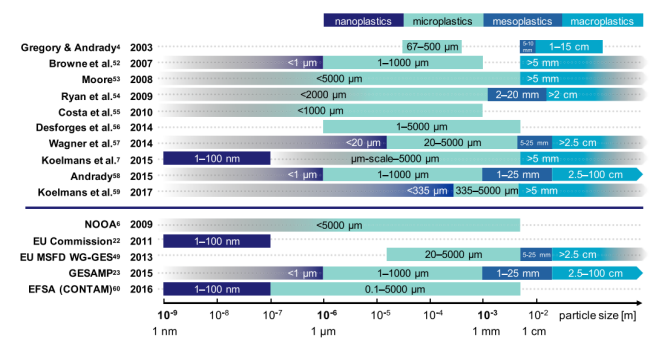
\includegraphics[width=\linewidth]{Figures/TetraTech.png}
		\caption[MP Size Classes]{Classifications of nano, micro, meso, and macro plastics.}
		\label{fig:TetraTech}
	\end{figure}
	It is useful to begin by establishing what exactly microplastics are defined as, and this paper does this by describing the classifications of and terminology used to describe microplastics. This project primarily discusses microplastics and nanoplastics, and thus these definitions were used to ensure consistency in the terms used. In addition to this, the paper discusses the distribution of microplastics among size classifications, indicating that smaller microplastics are more numerous than larger ones, with a continual increase in quantity as the size classification decreases. In this project, the net obtained had a somewhat large pore diameter of 300 microns, thus there will likely be many microplastics not captured by the filter in the device. Despite this disadvantage, 300 microns is the standard pore diameter of manta trawls used in many other studies referenced in this project for the purposes of modeling plastic collection, and thus using the same filter specification will increase the congruence between modeled effectiveness and real-world effectiveness.
	\subsubsection*{Microplastic Contamination in Freshwater Environments: A Review, Focusing on Interactions with Sediments and Benthic Organisms
	}
	This study focused on compiling and analyzing data from previous studies on the concentration of microplastics within various rivers and other bodies of water. The study also discussed the different units of measurement used by the various studies on the subject and attempted to reconcile and compare some of them, as currently plastic quantities are measured by weight, particles per unit of area, particles per unit of volume, and total number of particles. Overall, this lack of standardization slows down progress in measuring microplastics and mitigating their negative effects, and harms the study of microplastics as a whole. In addition, this study examined the ecotoxicology of microplastics and their ways of accumulating in benthic areas \cite{BellasiBenthic}.
	In this project, the data from this study was used primarily in the rationale, for explanations of the effects of microplastics on the environment, and for standardization of measurement for the modeling of the product’s effectiveness. Due to this paper illustrating the differences in measurement systems across studies, special care was taken to ensure congruence in units of measurement throughout this study in order to ensure accuracy. In addition, this study helped with the explanation of microplastics’ effects on benthic sedimentary systems, where they can constitute up to 3\% of sediments by weight. Benthic organisms are disproportionately affected by microplastics due to their high consumption of high density plastics which fall into the benthic zone and become mixed with naturally occurring sediment to be consumed. 
	
	\subsubsection*{Vertical Distribution of Microplastics in the Water Column and Surficial Sediment from the Milwaukee River Basin to Lake Michigan}
		\begin{figure}[H]
		\centering
		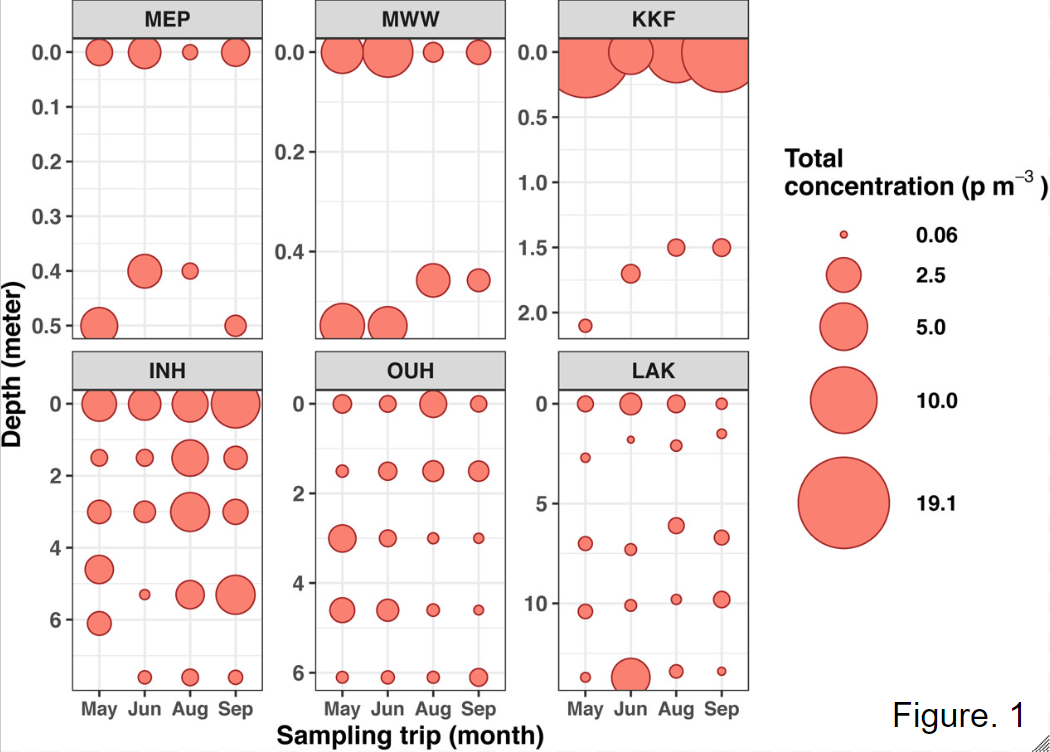
\includegraphics[width=0.8\linewidth]{Figures/DepthDistribution.png}
		\caption[Vertical MP Distribution]{Depth distributions of microplastics in various areas of the Milwaukee River basin. Here, the bottom-most measurements of the MEP samples were used primarily, along with the lowest measurements of MWW, INH, and LAK for comparison of benthic microplastic concentrations across various areas.}
		\label{fig:VerticalDepthDist}
	\end{figure}
	This study focused on the vertical distribution of microplastics throughout the water column of multiple rivers leading into Milwaukee Harbor and Lake Michigan. The levels of microplastics in each section of the water column were measured using Manta Trawls pulled at several depths below the water’s surface along with 1 sediment sample at each location, making for a total of 96 samples. The samples were separated according to the depth, location, and time that they were collected. The data collected is summarized in the table to the right. The data in the MEP graph was collected in the Milwaukee river in Milwaukee proper, MWW on the Menominee River, KKF in the Kinnickinnic River, INH at the innermost point of Milwaukee harbor, OUH at the outermost point of Milwaukee harbor, and LAK in Lake Michigan \cite{LenakerEtAlvertdist}.

	The data from this study gives a clear picture of the quantity of microplastics within the water column, specifically regarding the significant quantities of microplastics found in the benthic region of the water column throughout all parts of the year. This generally confirms that microplastics will be present during testing, and will provide a benchmark against which collection efficiency can be predicted and measured.
	
	
	\subsubsection*{Persistent Organic Pollutants: A Global Issue, A Global Response}
	This EPA article regards persistent organic pollutants (POPs), a class of chemicals typically produced by industrial processes which are capable of persisting within the environment for long periods of time after production. These chemicals are often highly harmful to humans and other wildlife\textemdash the most well-known example being DDT\textemdash and although regulations have significantly diminished the output of these chemicals into the environment, many POPs produced before this regulation still persist. In addition to these existing POPs, many POPs are either still created as byproducts of other industrial processes or are atmospherically transported over long distances from areas with looser regulations on their production. In addition to their already harmful impacts in their raw form, these chemicals also serve to multiply microplastics’ harmful effects by turning them into a vector for POPs that sorb onto them \cite{EPA}. 
	
	Here, this harm multiplication is the primary concern and rationale for removing microplastics from the sediment, as this transforms microplastics (especially the lines and fibers which most frequently “clog” bivalves’ digestive tracts) from detrimental to deadly. Just as POPs can sorb to microplastics, they can be leached off inside of living organisms\textemdash bioaccumulating with time to magnify the impacts which even trace amounts of POPs can have. This bioaccumulation combined with several other harmful effects caused by microplastics make them a prime threat to biodiversity and the environment, necessitating their active removal from the environment.
	
	
	\subsection{Microplastic and Sediment Transport}
	\subsubsection*{Numerical study on the dissipation of water waves over a viscous fluid-mud layer}
	This research paper by Deng et al. gives insight into the transport of sediment through the water column due to the forces of waves, with simulations modeling the vorticity caused by these forces along with the subsequent motion imparted to benthic sediment. The results of these simulations lend credence to the idea that a device capable of filtering only the bottom few centimeters of the water column could significantly impact the quantity of microplastics carried in the benthic boundary currents of rivers and lakes. As seen here, surface waves and pelagic currents create significant vorticity in these regions, creating conditions such that benthic sediment and the associated microplastics can be re-suspended after their initial deposition. This is the most relevant interaction within the water column, as this re-suspension gives microplastics the opportunity to be re-ingested into bivalves and other organisms\textemdash causing several problems \cite{Deng_Hu_Guo_Dalrymple_Shen_2017}.
	\begin{figure}[h]
		\centering
		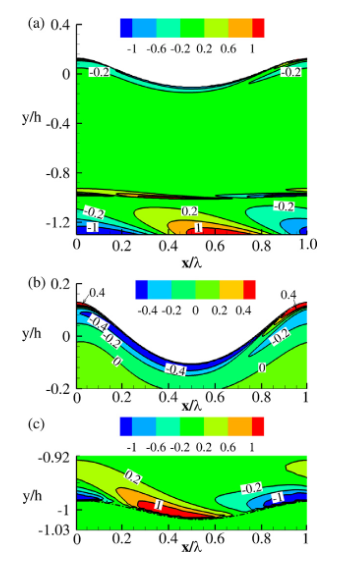
\includegraphics[width=0.5\linewidth]{Figures/RiverTurbulence.png}
		\caption[Benthic Turbulence Models]{Models of turbulence due to surface currents and waves in the benthic region}
		\label{fig:TurbulenceBenthic}
	\end{figure}
	Note here the bottom diagram of figure \ref{fig:TurbulenceBenthic} depicting the region within the bottom 0.08\% of the water column. As shown, essentially all of the currents’ impact on the muddy sediment is concentrated within the bottom half of this region, meaning that a device collecting only from this region would be well-situated to remove the vast majority of benthic plastics. In a place like the Milwaukee River where depths average roughly 0.4 meters as seen in figure \ref{fig:riverCrosssec}, this means that collecting from the bottom 1.6 centimeters of the river is sufficient to access the vast majority of sedimentary transport. In the extreme example of something as large as the Mississippi River, the bottom 12 centimeters would need to be collected for this same result, but given that the agitated sediment eventually falls down it is possible to collect a similar proportion of sedimentary transport simply by using multiple devices downstream of each other.
	
	
	\subsection{Biotic Microplastic Selection}
	
	\subsubsection*{Separating the Grain from the Chaff: Particle Selection in Suspension- and Deposit-Feeding Bivalves}
	The class Bivalvia is incredibly diverse, populous, and ecologically important\textemdash with nearly 10,000 extant species, populations as high as 1.5 million per acre of seabed, and a critical role in limiting the proliferation of pelagic and benthic algae along with reducing turbidity. This study examines the class, and particularly their unique ability to individually differentiate particles in the benthic flow in order to feed on the algae and other biomass within. Though many variations exist, the study identifies several general methods of bivalve feeding\textemdash one of which, siphoning, was a primary inspiration for the form of the device proposed here. 
	\begin{figure}[h]
		\centering
		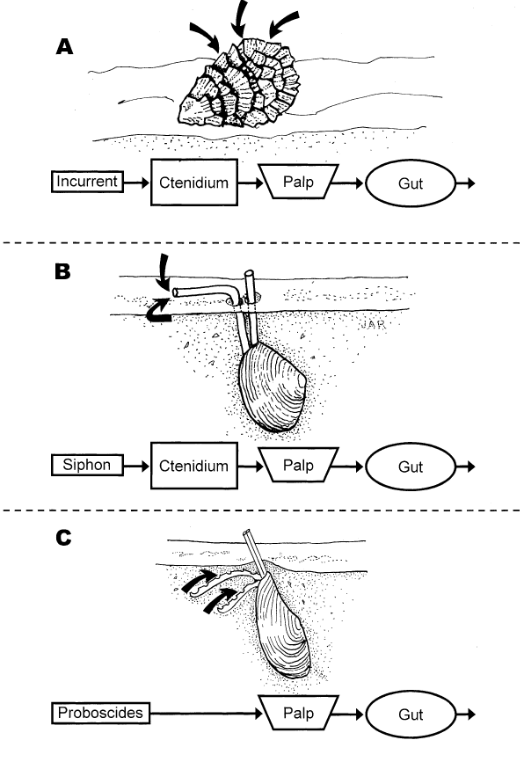
\includegraphics[width=0.5\linewidth]{Figures/BivalveInspo.png}
		\caption[Bivalve Filter-Feeding Techniques]{A visual summary of the three primary methods by which bivalves separate biomass from benthic flow in order to feed.}
		\label{fig:SiphonInspo}
	\end{figure}
	Noted in section B of figure \ref{fig:SiphonInspo}, the siphon intakes water through a small tube facing into the flow of a waterway, moves it underwater, filters it for nutrients and biomass, then ejects faeces and pseudofaeces through an exit siphon which carries the material out of the sediment. This is very similar to the design of the device presented here, and the siphon mode of feeding found in nature indicates that such an approach could be an optimal method for unobtrusively collecting benthic flow. 
	
	\subsubsection*{Particle Selection in Suspension-Feeding Bivalves: Does One Model Fit All?}
	
	Bivalves, one of the primary inspirations for this study, are marked in large part by their ability to differentiate similar sestons within the benthic flow, then individually select these particles and decide whether to ingest or reject them. As of this study’s writing, the exact methods by which this occurs are unknown, despite a significant body of work regarding the matter\textemdash but understanding this ability is crucial to creating a device which aims to do essentially the same thing. The 2020 study examines the role of proteins called lectins in this process, and determined that particle selection is in large part determined by the exterior characteristics of particles as opposed to intrinsic factors like density, implying that if something like a microplastic becomes bound to particles typically consumed by bivalves, it could be misidentified and subsequently consumed. 
	The ways in which particles are selected by bivalves is important here primarily because identifying bivalves’ selection criteria can help in identifying the few easily differentiable qualities between microplastics, sediments, and other sestons\textemdash thus enabling the creation of a device which dynamically detects these differences. Here, the knowledge that exterior chemical composition is a key factor in bivalve selection, along with the fact that different chemicals emit different light spectra when irradiated helped spur the development of the general system used in the device described by this project.
	
	\subsubsection*{Postingestive selection in the sea scallop, Placopecten magellanicus (Gmelin): the role of particle size and density}
	Bivalve particle selection typically occurs in two ways\textemdash first through pre-ingestive selection by which bivalves decide whether to ingest particles based upon exterior chemical factors or to reject as pseudofaeces, then second through post-ingestive selection inside of the stomach and intestine. Here, selection is primarily focused on ensuring that all ingested particles are properly broken down before entry into the intestines and ejection as feces. This occurs by circulating fluid through the stomach, with the stomach walls being made of tightly folded material which only allows particles below a certain size to enter. If particles are too large, they then remain in the stomach until bacteria and the constant circulation can break them down into digestible portions. Given enough time, however, due to the imperfect nature of the stomach, larger particles can move into the intestine if they are not too large. This makes microplastic ingestion a serious issue, as the particles ingested are almost entirely unable to be digested by the bivalve, filling up the stomach and, if severe enough, making the bivalve stop eating entirely in a perpetual wait for the plastic to be digested \cite{Brillant_MacDonald_2000}.
	\linebreak
	Interestingly, though published before the discovery of microplastics as a widespread environmental pollutant, this study used small plastic beads as an analog to the sestons consumed by oysters\textemdash discovering how easily bivalves can consume microplastics coated in environmental media before anyone had imagined exactly the damage which such consumption wrought on benthic ecosystems. Here, this serves as the primary rationale for the project and an explanation of exactly why it is so important to remove microplastics at the source.
	
	\subsection{Artificial Microplastic Selection}
	\subsubsection*{ Identification of different plastic types and natural materials from terrestrial environments using fluorescence lifetime imaging microscopy}
	The greatest challenge which arises when attempting to remove microplastics from benthic flow while in-situ is that of identification. More than any other section of the water column, the benthic region is full of sestons which are of very similar size, density, and shape to microplastics\textemdash making most methods of removal wholly inadequate to accurately identify the different particles. Coupled with the fact that unobtrusive and in-situ removal of these particles must occur underwater, a novel method must be used to accomplish this. This study presents that method, whereby shining lasers near the UV range of light onto microplastics and other environmental particles allows for clear, rapid identification of the particles.
	\begin{figure}[h]
		\centering
		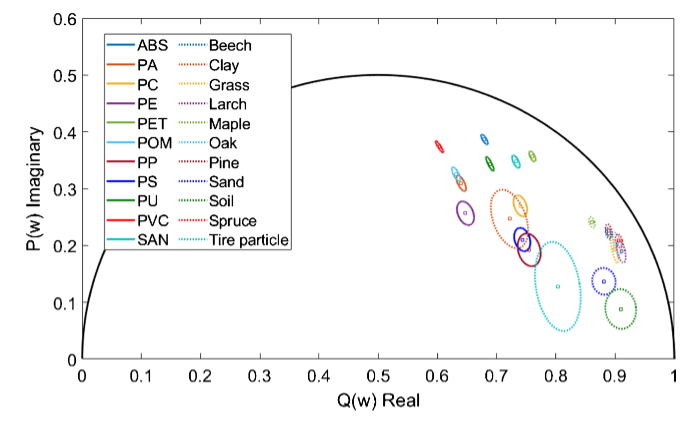
\includegraphics[width=1\linewidth]{Figures/Phasor.png}
		\caption[Phasor Plot \textemdash MPs and Organics]{This type of plot (a phasor plot) is read using polar coordinates beginning from the (0,0) point in the bottom left corner. The distance along the outer edge of the semicircle (as determined by intersecting a ray from (0,0) with the outer ring) measures the duration of fluorescence for a given particle, and thus the intensity with which it re-emits light.}
		\label{fig:Phasor}
	\end{figure}
	\begin{figure}[h]
		\centering
		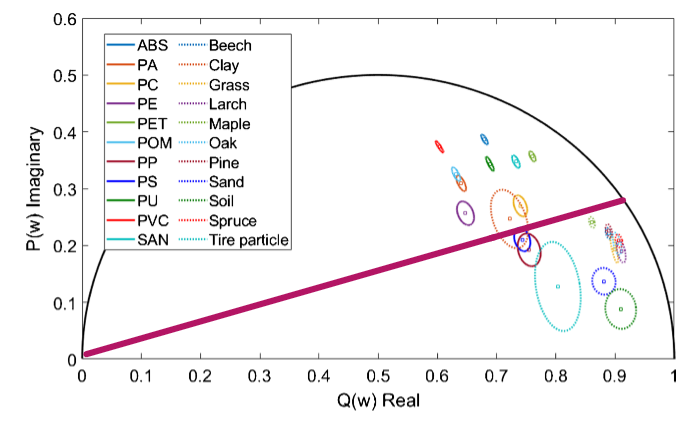
\includegraphics[width=1\linewidth]{Figures/PhasorAnnotated.png}
		\caption[Annotated: Phasor Plot \textemdash MPs and Organics]{The magenta line here denotes a clear divide between the fluorescence lifetimes of biotic and abiotic particles.}
		\label{fig:PhasorAnnotated}
	\end{figure}
	
	Using FD-FLIM (Frequency-Domain Fluorescence Lifetime Imaging Microscopy), the authors of this study identified that a clear distinction can be drawn between a large number of environmental sestons and artificial sestons\textemdash where as shown in the phasor plot above, all plastics (which were examined) except for PS (PolyStyrene) and PP (PolyPropylene) can be divided from all biotic particles (which were examined) except for grass by the magenta line drawn over the phasor plot. Various other factors impact exactly how the measurements are situated inside of the circle (positions are truly formed through the linear combination of each particles’ constituent molecules’ position on the outside edge of the circle), but these are not important for the purposes of this project. Here, the most important aspect of the plot is that due to the clear divide between plastics and biotic materials, there is also a clear distinction between the amount of light reemitted when viewed by a camera. 
	
	\begin{figure}[h]
		\centering
		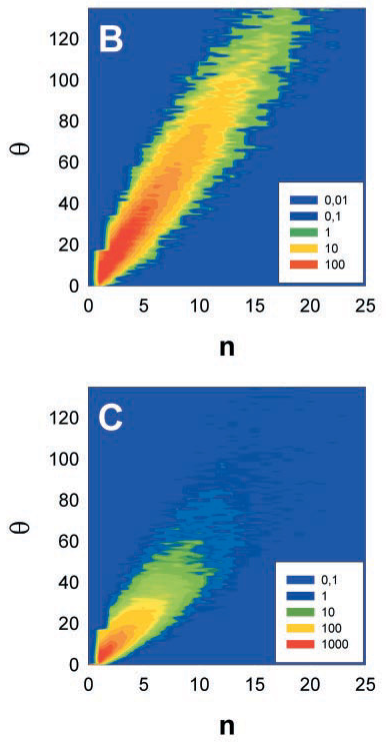
\includegraphics[width=0.5\linewidth]{Figures/FluorescenceCorrelation.png}
		\caption[Fluorescence Lifetime and Intensity Correlation]{This figure from \cite{Palo_Brand_Eggeling_Jäger_Kask_Gall_2002} shows the correlation between theta and n for various dyes ($\theta$ = fluorescence lifetime in ns, n = photon count). $n \propto \theta$}
		\label{fig:FluorescenceCorrelation}
	\end{figure}
	
	This is demonstrated in figure \ref{fig:FluorescenceCorrelation} from \cite{Palo_Brand_Eggeling_Jäger_Kask_Gall_2002}. Note also that the cameras do not actually measure fluorescence lifetimes, but that fluorescence intensity is highly correlated with fluorescence lifetimes as seen in figure \ref{fig:FluorescenceCorrelation}. Although the results in figure \ref{fig:FluorescenceCorrelation} \textbf{do not actually prove that there exists a similar correlation with microplastics}, experimental examination of fluorescence intensity does appear to show a correlation with the fluorescence lifetimes found in \cite{Wohlschläger_Versen_Löder_Laforsch_2024} for microplastics and organic particles. It is possible that such a correlation holds for most or all other classes of particles, but no evidence has been found to support this broader conclusion.
	
	\begin{figure}[h]
		\centering
		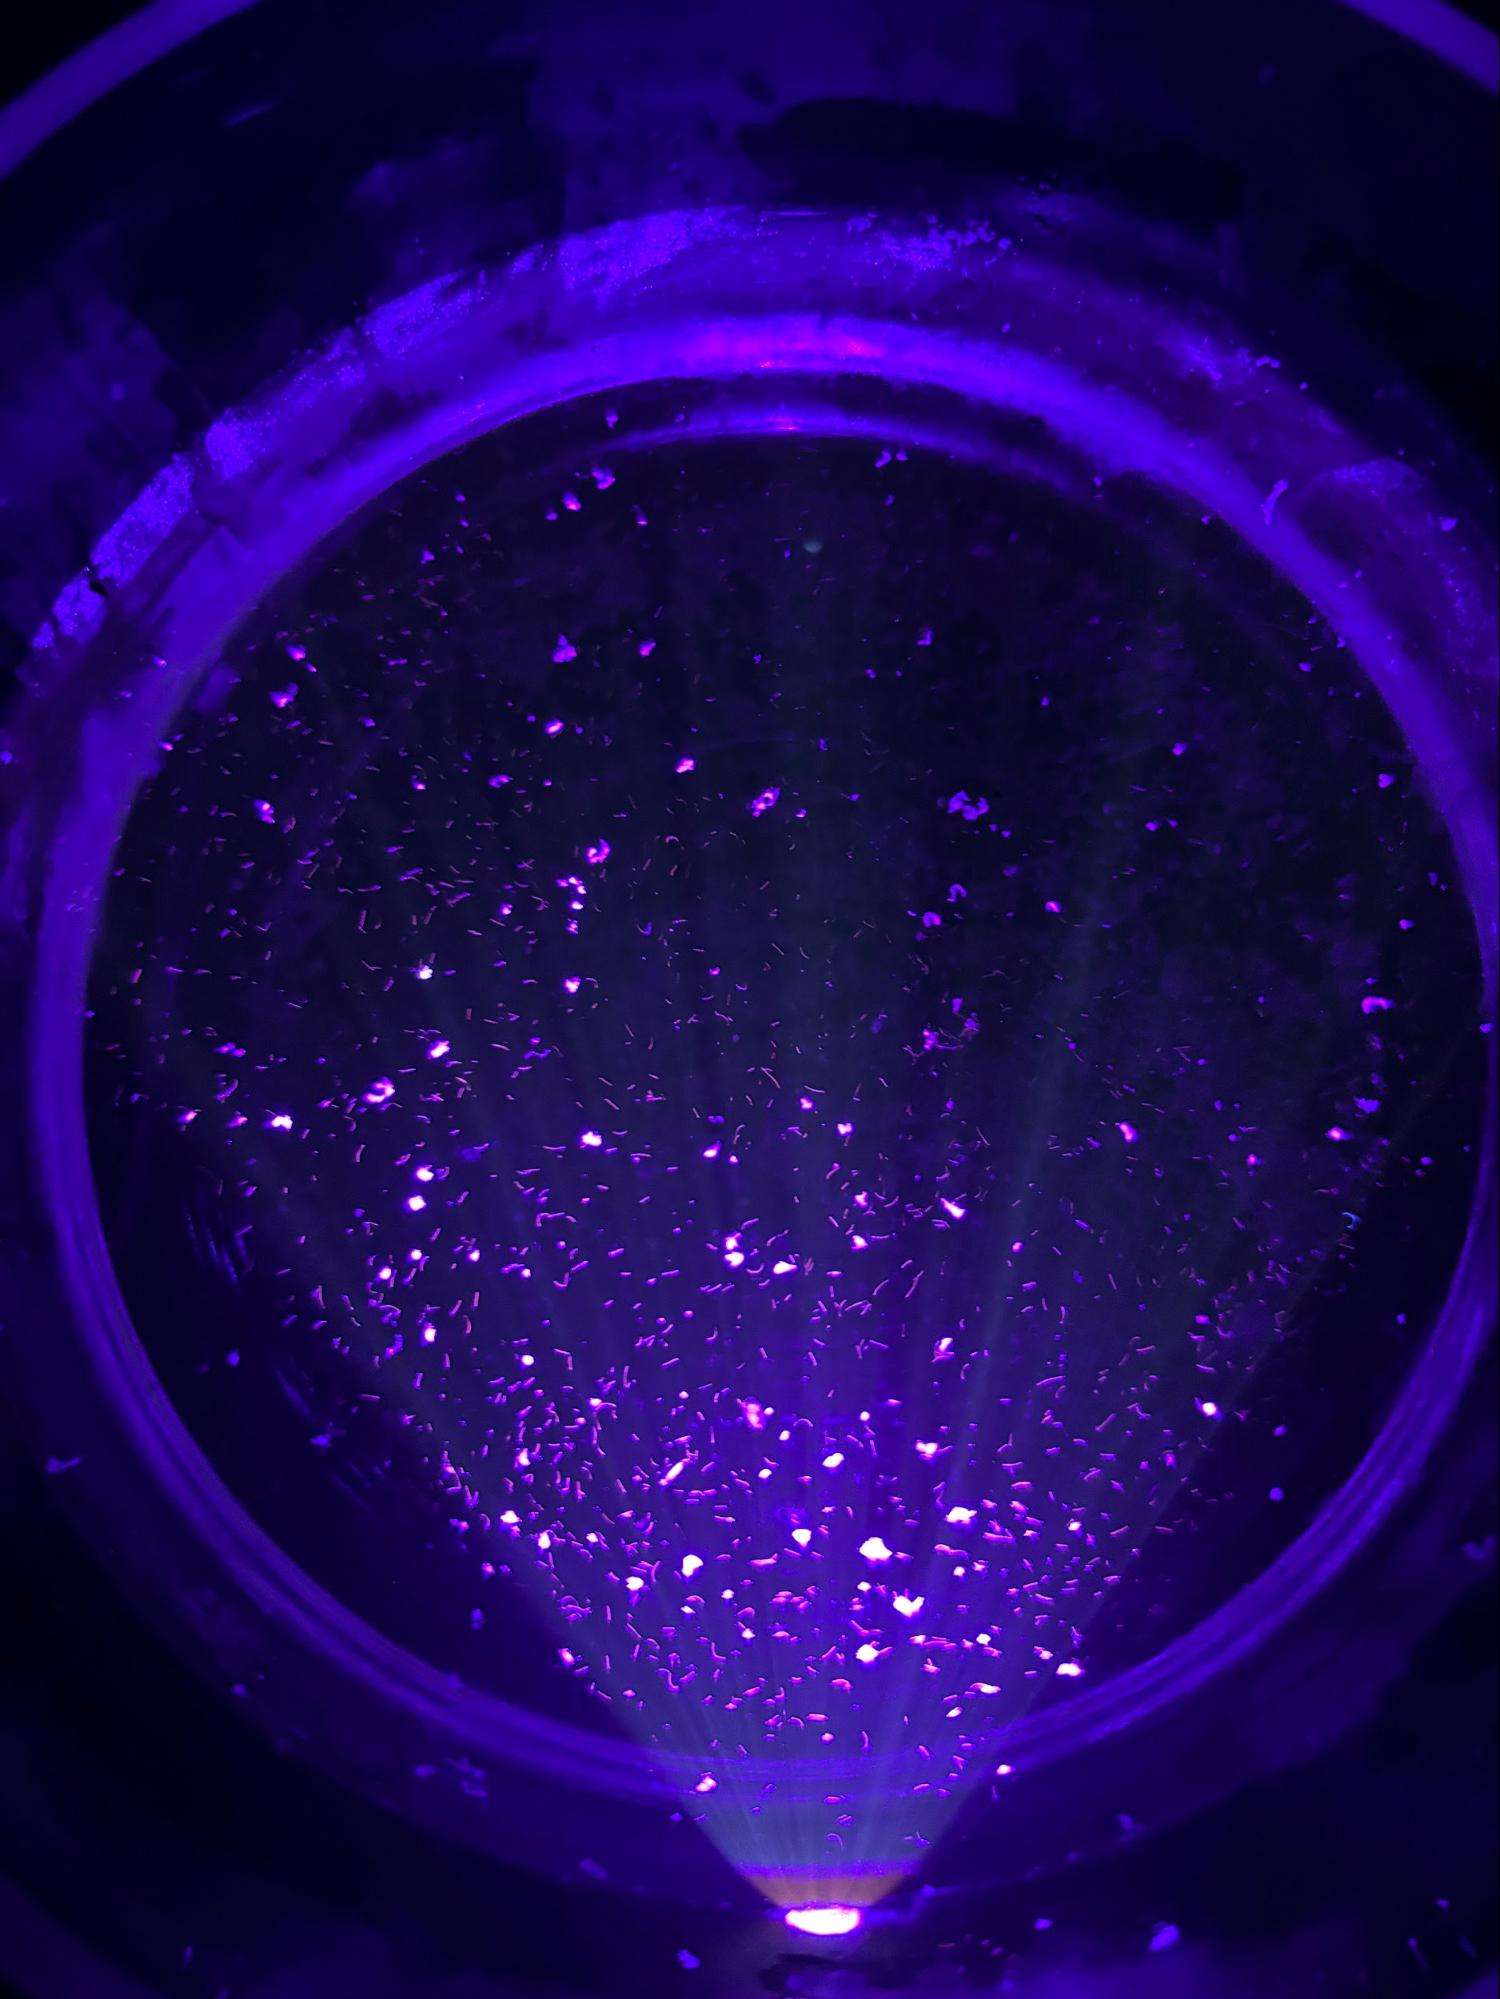
\includegraphics[width=1\linewidth]{Figures/FluorescedMPs2}
		\caption[Microplastics Fluorescing]{This image shows microplastics collected from the Milwaukee River in \cite{Isahaku}. Using a 405 nm linear laser beam, the microplastics glow in the shorter wavelengths of the visible spectrum while other particles glow with longer wavelengths. Here, very few of these other particles can be seen.}
		\label{fig:FluorescedMPs}
	\end{figure}
	
	\section{Procedure}
	
	\subsection{Overview}
	The primary functionality of the proposed device involves selectively filtering benthic river currents in order to primarily collect microplastics while avoiding collection of other sestons within the benthic region of rivers. Filtering these benthic microplastics is far more difficult than filtering most other microplastics, with the three primary difficulties being that: 
	\begin{enumerate}
		\item The benthic region of rivers contains a far greater quantity of sestons than the pelagic and demersal regions due to benthic boundary circulation.
		\item The set of benthic sestons comprises a significant number of micro and meiobenthos which are very important to benthic ecosystems, and thus must not be harmed. 
		\item Microplastics are very difficult to distinguish reliably from other benthic sestons due to their great similarity to various types of sediment with regard to their density, shape, size, and other qualities.
	\end{enumerate}
	These three difficulties make selective removal of microplastics very difficult, especially if attempted continuously, and thus a solution which removes these particles by indiscriminately filtering continuously selected discrete samples of water is proposed. Here, inspiration is taken from bivalves\textemdash a class capable of selectively filtering biomass out of a large range of ingested sestons which include microplastics, sediments, and other particles. These organisms’ digestive systems are highly discretized, with specialized organs separating the ingested sestons on a particle-by-particle basis. It is not yet known exactly which criteria bivalves use for this discrete selection, thus it is near impossible at the current moment to accurately replicate their digestive systems in an accurate manner. This is an active field of research, and a key area of future study will likely be how to replicate these systems once more is revealed on their inner functionings. 
	
	\subsection{Methods}
		Given the lack of research on methods by which bivalve seston selection can be artificially replicated, a novel method must be used to achieve selection. Here, the properties of microplastics must be leveraged in order to remove them most efficiently\textemdash with the most relevant property being their autofluorescence after excitation from violet light. Recent advancements in the field of FD-FLIM (Frequency-Domain Fluorescence Lifetime Imaging Microscopy) have established that microplastics will fluoresce after excitation \cite{Wohlschläger_Versen_Löder_Laforsch_2024}, with the fluorescence spectra being dependent on the type of microplastic\textemdash meaning that a camera aimed directly at a plastic which is actively being excited can detect not only how many particles exist in a sample, but also which types of plastic exist therein. In addition to plastics, organic materials and sediment particles (clay, sand, soil) also have their own relatively consistent fluorescence spectra, meaning that if a clear separation can be made between each of these categories, they can be identified and removed individually. 
\begin{figure}[h]
	\centering
	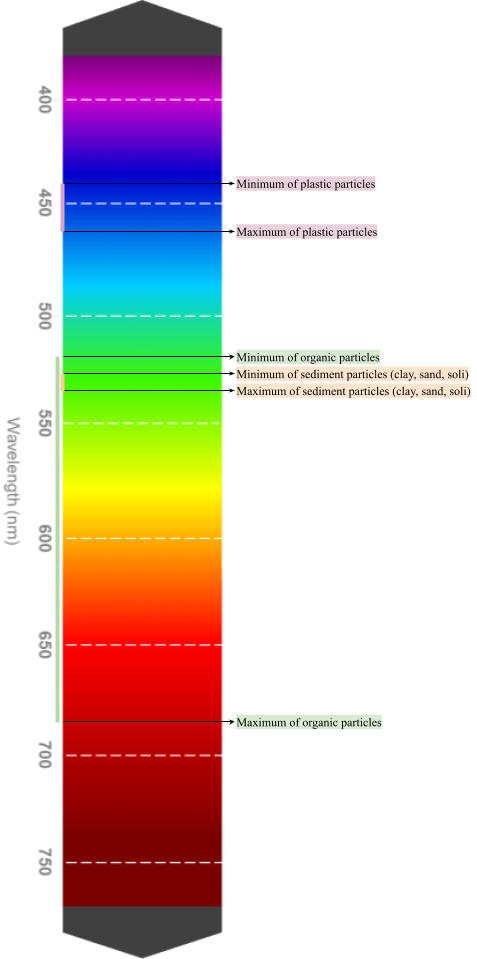
\includegraphics[width=0.6\linewidth]{Figures/MPSpectrum}
	\caption[MP and Organic Re-emission Wavelengths]{This figure illustrates the different reemission wavelengths of microplastics and a few other notable particle classes. The chart itself was compiled by the author, and the data used to create it is found in the supplementary materials of \cite{Wohlschläger_Versen_Löder_Laforsch_2024}.}
	\label{fig:SestonSpectra}
\end{figure}
		This, notably, means that the proposed device could be used not only to remove microplastics, but any other particle class with distinct fluorescence spectra\textemdash though separation with the exact device created here is likely to be limited to the aforementioned classes due to relatively low camera resolution. After taking an image, the camera’s data can then be processed by a microcomputer such as a Raspberry Pi in order to identify the particles that exist within the sample, and make a decision as to whether or not the sample should be filtered. As aforementioned, it is incredibly difficult to accurately and selectively filter only one type of particle from a sample, therefore instead of attempting to remove individual particles once they are detected, the device can instead use a water velocity sensor in the form of a simple turbine to determine the rate of particle movement through the device. Using this data, it can be determined exactly when each particle reaches any arbitrary distance through the device. This allows us to then divert the fluid flow into one of two channels\textemdash with one channel simply exiting the device and returning fluid back into the flow of the river, and the other leading particles through an indiscriminate filter which removes all suspended particles from the channel. 
	
	\subsection{Design Overview}
	The design of the device used to accomplish the objectives of selectively filtering particles can be effectively split into four parts: henceforth called the inlet, processor, selector, and outlet. These parts combined with a compute module, power generation, and microplastic containment module complete the device, allowing for continuous filtration of selected particles in the benthic region. This section gives a brief overview of the functions and design of each of these sections, for a more detailed description of each part’s construction, design, and assembly refer to  section \ref{subsec:TechDesign}.
	
	\subsubsection{Inlet}
	Perhaps the simplest of the sections, the inlet’s only purpose is to collect water flowing in the benthic region and transport it to the processor\textemdash meaning that its structure is similarly basic. The inlet transports water from the bottom three centimeters of the water column through a 30x30mm inner diameter square tube, bringing it to the processor in a tube of the same shape.
	
	\begin{figure}[h]
		\centering
		
\includegraphics[width=1\linewidth]{Figures/InletInSitu}
		\caption[Inlet 2D Model]{This figure illustrates how the inlet piece of the device described here emerges above the riverbed to collect benthic flow.}
		\label{fig:InletInSitu}
	\end{figure}
	
	\subsubsection{Processor}
	The most complex of the sections is the processor, and it handles all of the work of identifying particles in tandem with the compute module. A cross-section of the processor is shown to the right, with the 30x30mm square tube at the bottom-center, the two 405 nm lasers placed in the angled cavities at the top, and the two RPI Camera Module V2 cameras on each side of the device at the bottom left and right. The lasers shine through a thin 8mm flat cavity, angled at 55° above the horizontal so that their 110°-wide beams shine directly downwards and outwards to avoid intrusion into the 6mm wide cavity through which the cameras view the tube, and illuminate a thin section\textemdash causing each particle to re-emit light at a certain intensity and wavelength. 
		\begin{figure}[h]
		\centering
		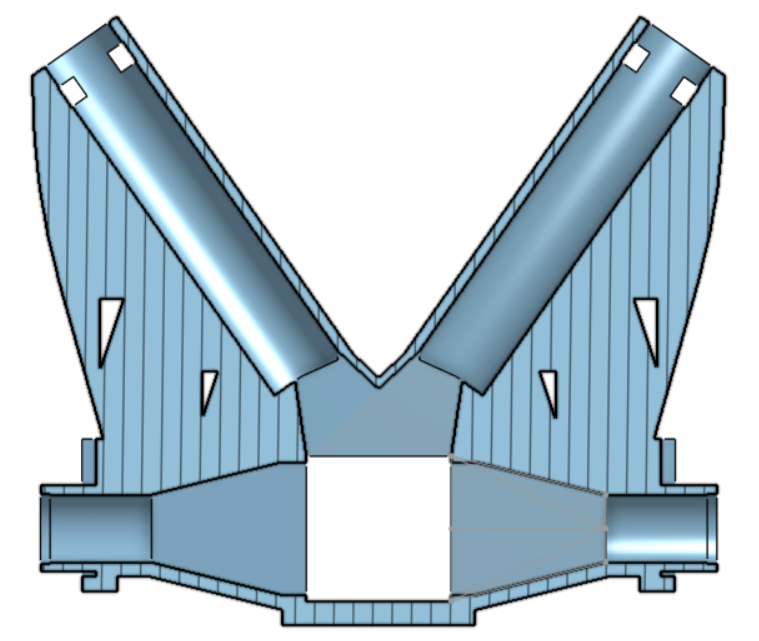
\includegraphics[width=1\linewidth]{Figures/ProcessorCrosssection}
		\caption[Processor Cross-section]{A cross-section of the processor. The central square is the tube which water flows through, lasers shine inwards from the two slanted cavities, and cameras look inwards from the two cavities on the left and right side.}
		\label{fig:ProcessorCrosssec}
	\end{figure}
	This is then captured by the dual cameras, which capture footage at roughly 215 fps to ensure capture of particles traveling at speeds as high as 2 m/s. The data captured by the cameras is then transferred to the RPI compute module for processing\textemdash after which the RPI sends commands to the servo housed within the selector section to, as the name suggests, select which particles should be filtered and which should be expelled. 
	\begin{figure}[h]
		\centering
		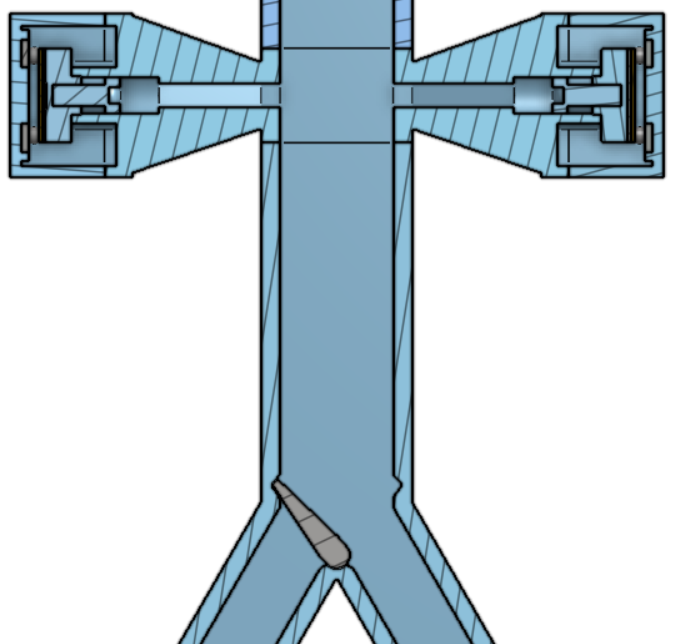
\includegraphics[width=1\linewidth]{Figures/OverheadCrosssection}
		\caption[Selector Cross-section]{An overhead cross-section of the processor and selector. The processor can be seen as the two side-mounted boxes near the top of the figure, and the selector's flipper is shown in gray near the bottom.}
		\label{fig:OverheadCrosssec}
	\end{figure}
	
	\subsubsection{Selector}
	The selector is a relatively simple mechanism attached directly to the outlet which consists of a single servo motor attached to a flipper which controls the direction which water travels. As shown, the gray flipper rotates on the servo, with figure \ref{fig:OverheadCrosssec} showing the flipper in the default position which allows water to travel through the port-side channel and back out to the river without disruption. If switched to the starboard side, the flipper will divert the water into a channel with a filter and collection mechanism, removing any diverted sestons from the flow.
	
	\subsubsection{Outlet}
	Nearly as simple as the inlet, the outlet consists of two channels which transfer water upwards above the sediment and expel all non-diverted sestons back into the general river flow.
	
	\subsection{Technical Design and Construction}
	\label{subsec:TechDesign}
	\subsubsection{Design Principles}
	
		Throughout every part of the device’s design, manufacture, and operation, three central principles and ideas have been maintained in order to guarantee consistent and effective design. These are as follows.
	\begin{enumerate}
		\item Do not intrude on nature.
		\subitem The fundamental goal behind this device is to aid ecosystems at risk from microplastics and anthropogenic pollution\textemdash thus any successful device must necessarily be one which does not run counter to these ideals. Because of this, every piece of the device has been designed so as to be minimally intrusive to nature, with minimal exposure to the biotic elements of the environment. This was critical to the design decision to bury the majority of the device under several inches of sediment, ideally preventing fish, benthos, and other organisms from interacting with the device as much as possible.
		\item Prioritize protection over speed and efficiency.
		\subitem Without a doubt, microplastics could be removed from sediment far more quickly than with the method proposed here, namely by dredging, separating, and re-depositing sediment. Much study has already been done on how to most efficiently conduct each of these steps, and many separation techniques have been found which can quickly separate microplastics from sediment in a lab, however, these have the fundamental and as-of-yet unresolved issue of harming or potentially killing the organisms within the benthic sediment. This makes nearly all of these methods completely infeasible for application within the realm of environmental protection, though potentially useful for more lucrative industrial applications in products like concrete which use sediment. 
		\item Design to maximize simplicity, versatility, and robustness.
		\subitem For this and any other devices which must survive significant periods of time while in environments where humans will have limited ability to repair and access them, simplicity and robustness are key to a successful final product. If a design is too complex to survive the benthic riverine environment long-term, unable to adjust to changing conditions, or lacking the redundancy necessary to survive part failures, it will quickly fail. To combat this, the device designed here attempts to exclusively use the strength of its own parts to stay together\textemdash avoiding materials like glue which create extra opportunities for failure, and ensuring that any part failure will be due to a stress which is so overwhelming that the material the device is made of (minimum 5mm/$\approx$25 layer thick, 100\% infill 3D printed PLA) will itself break. 
		
		
		
	\end{enumerate}
	\subsubsection{Materials}
		The vast majority of the device is constructed of 3D-printed PLA, with several other components used to complete the device and perform specific tasks. Following is the list and quantities of these materials.
	
	\begin{enumerate}

	\item 1.75 mm PLA Plastic Filament (1.2 kg w/o supports)
	\item 405 nm wavelength linear laser (x2)
	\item IP68 Servo
	\item EK1894 5v DC Motor
	\item 50W Solar panel
	\item 12V LiPo Overcharge prevention circuit
	\item 15,000 mAh Li-Po battery
	\item Raspberry Pi CM4
	\item Raspberry Pi CM4 I/O Board
	\item Raspberry Pi Pico 1 W
	\item Raspberry Pi Camera module v2 (x2)
	\item RPI Cam v2 M12 lens mount (x2)
	\item 25 mm M12 camera lens (x2)
	\item RPI Cam v2 ribbon cable (x2)
	\item 12v$\rightarrow$5v Buck regulator
	\item 12v Solid state relay
	\item Assorted wires
			 
	\end{enumerate}
	
	\begin{figure}[h]
		\centering
		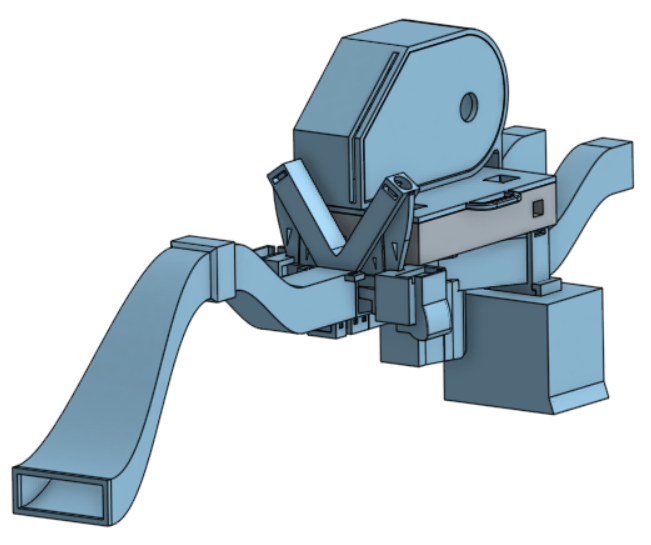
\includegraphics[width=1\linewidth]{Figures/CADFull}
		\caption[Complete 3D Model]{The complete CAD model of the device.}
		\label{fig:FullCAD}
	\end{figure}
	\subsubsection{Design and Construction}
		As aforementioned, the design of the device described here can be seen as a sequence of elements through which particles and water flow\textemdash and thus, this is how the design will be described in the following section. Beginning with the inlet, each piece, its function, and the reasons for its design will be described, eventually arriving at the outlet in accordance with the path that microplastics take through the device. 
		\begin{figure}[h]
			\centering
			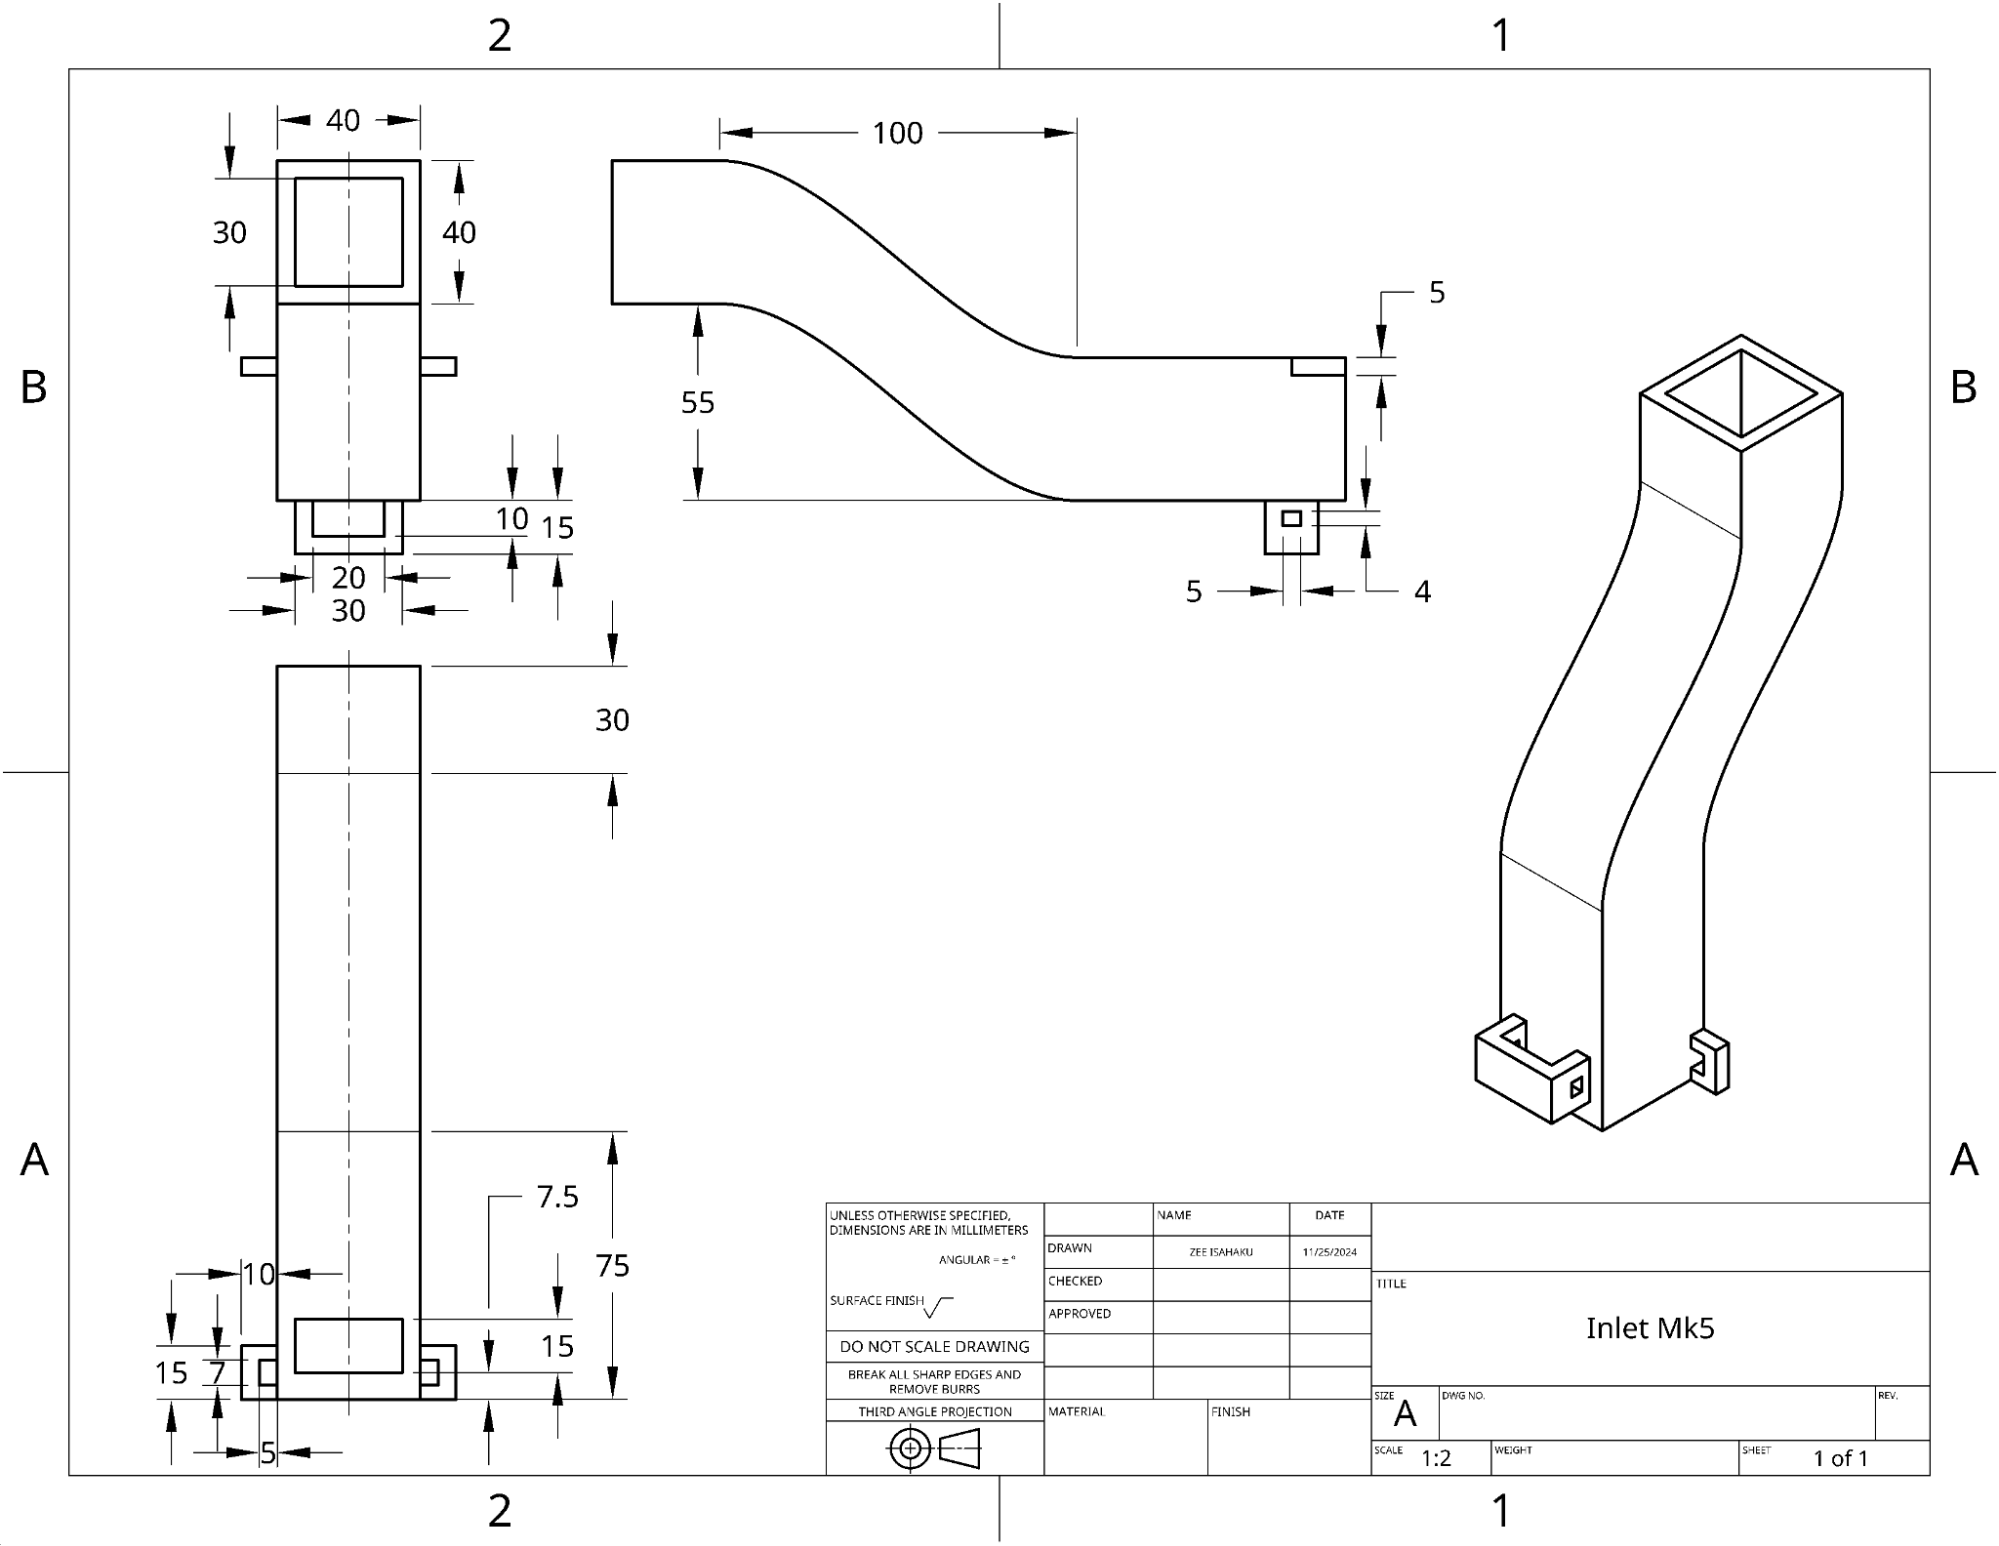
\includegraphics[width=1\linewidth]{Figures/TechInlet}
			\caption[Inlet Tech. Drawing]{Technical drawing of the inlet.}
			\label{fig:techinlet}
		\end{figure}
			The first piece of the device is the inlet, which extrudes from the sediment by roughly 3 cm to capture the primary section of the benthic flow. Most of this flow is concentrated within this region, as benthic sediment particles are exclusively non-buoyant and thus are only transported by temporary periods of higher turbulence. This occurs constantly, with tiny portions of sediment being transported downstream by miniature turbidity caused by a non-uniform riverbed. This sediment-water mixture constantly pushes through the device, traveling down through the inlet then directly into the processor. 
		\begin{figure}[h]
			\centering
			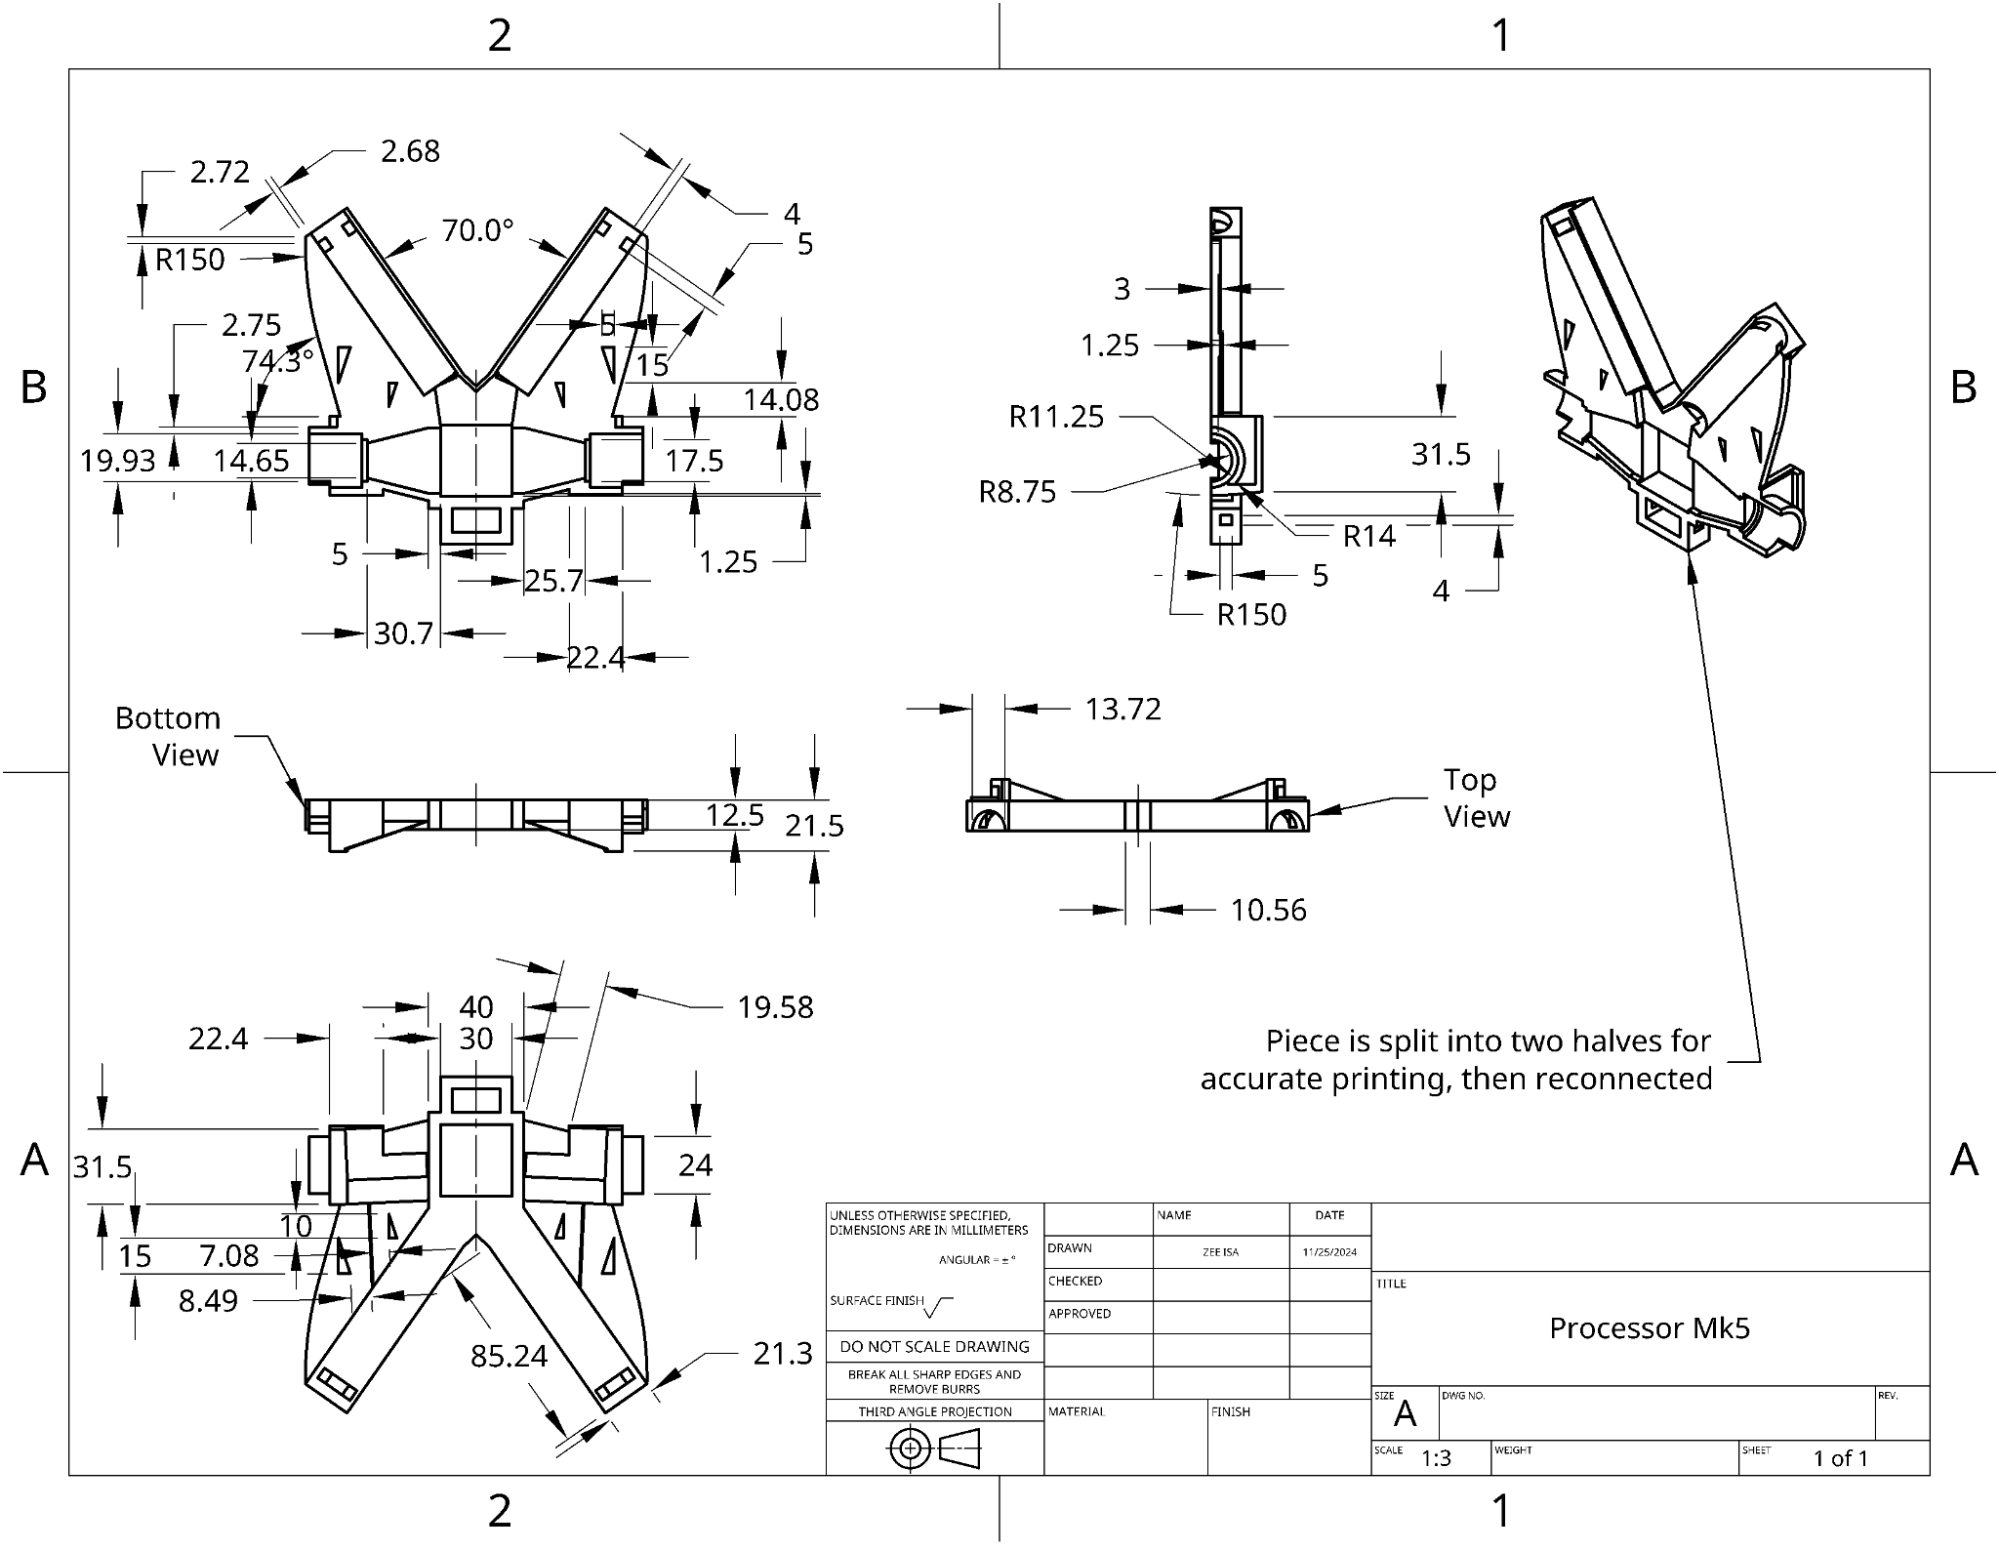
\includegraphics[width=1\linewidth]{Figures/TechProcessor}
			\caption[Processor Tech. Drawing]{Technical drawing of the processor.}
			\label{fig:techprocessor}
		\end{figure}
			The processor is the most complex portion of the device, being constructed of two halves which are bound together with epoxy and physical connectors to ensure that a proper connection is always maintained. The processor contains the two lasers which, together, illuminate the particles travelling through the device. The two lasers illuminate each particle from both sides equally, enabling both cameras to have a similar view of each particle and to send their data back to the compute module for analysis. As seen in the technical drawing, the cavity through which the cameras view the particles is only 6mm wide, ensuring that every capture has a very similar profile and that the linear lasers always light up the particles in the viewport. Near the bottom, on the left and right sides, there also exist connection points for the camera’s waterproof enclosure to ensure water doesn’t enter the cameras’ compartment and risk damaging them. To aid in this, the cameras’ circuit boards are also covered in epoxy so that any minor leaks, humidity, or other water intrusion doesn’t damage them. 
		\begin{figure}[h]
			\centering
			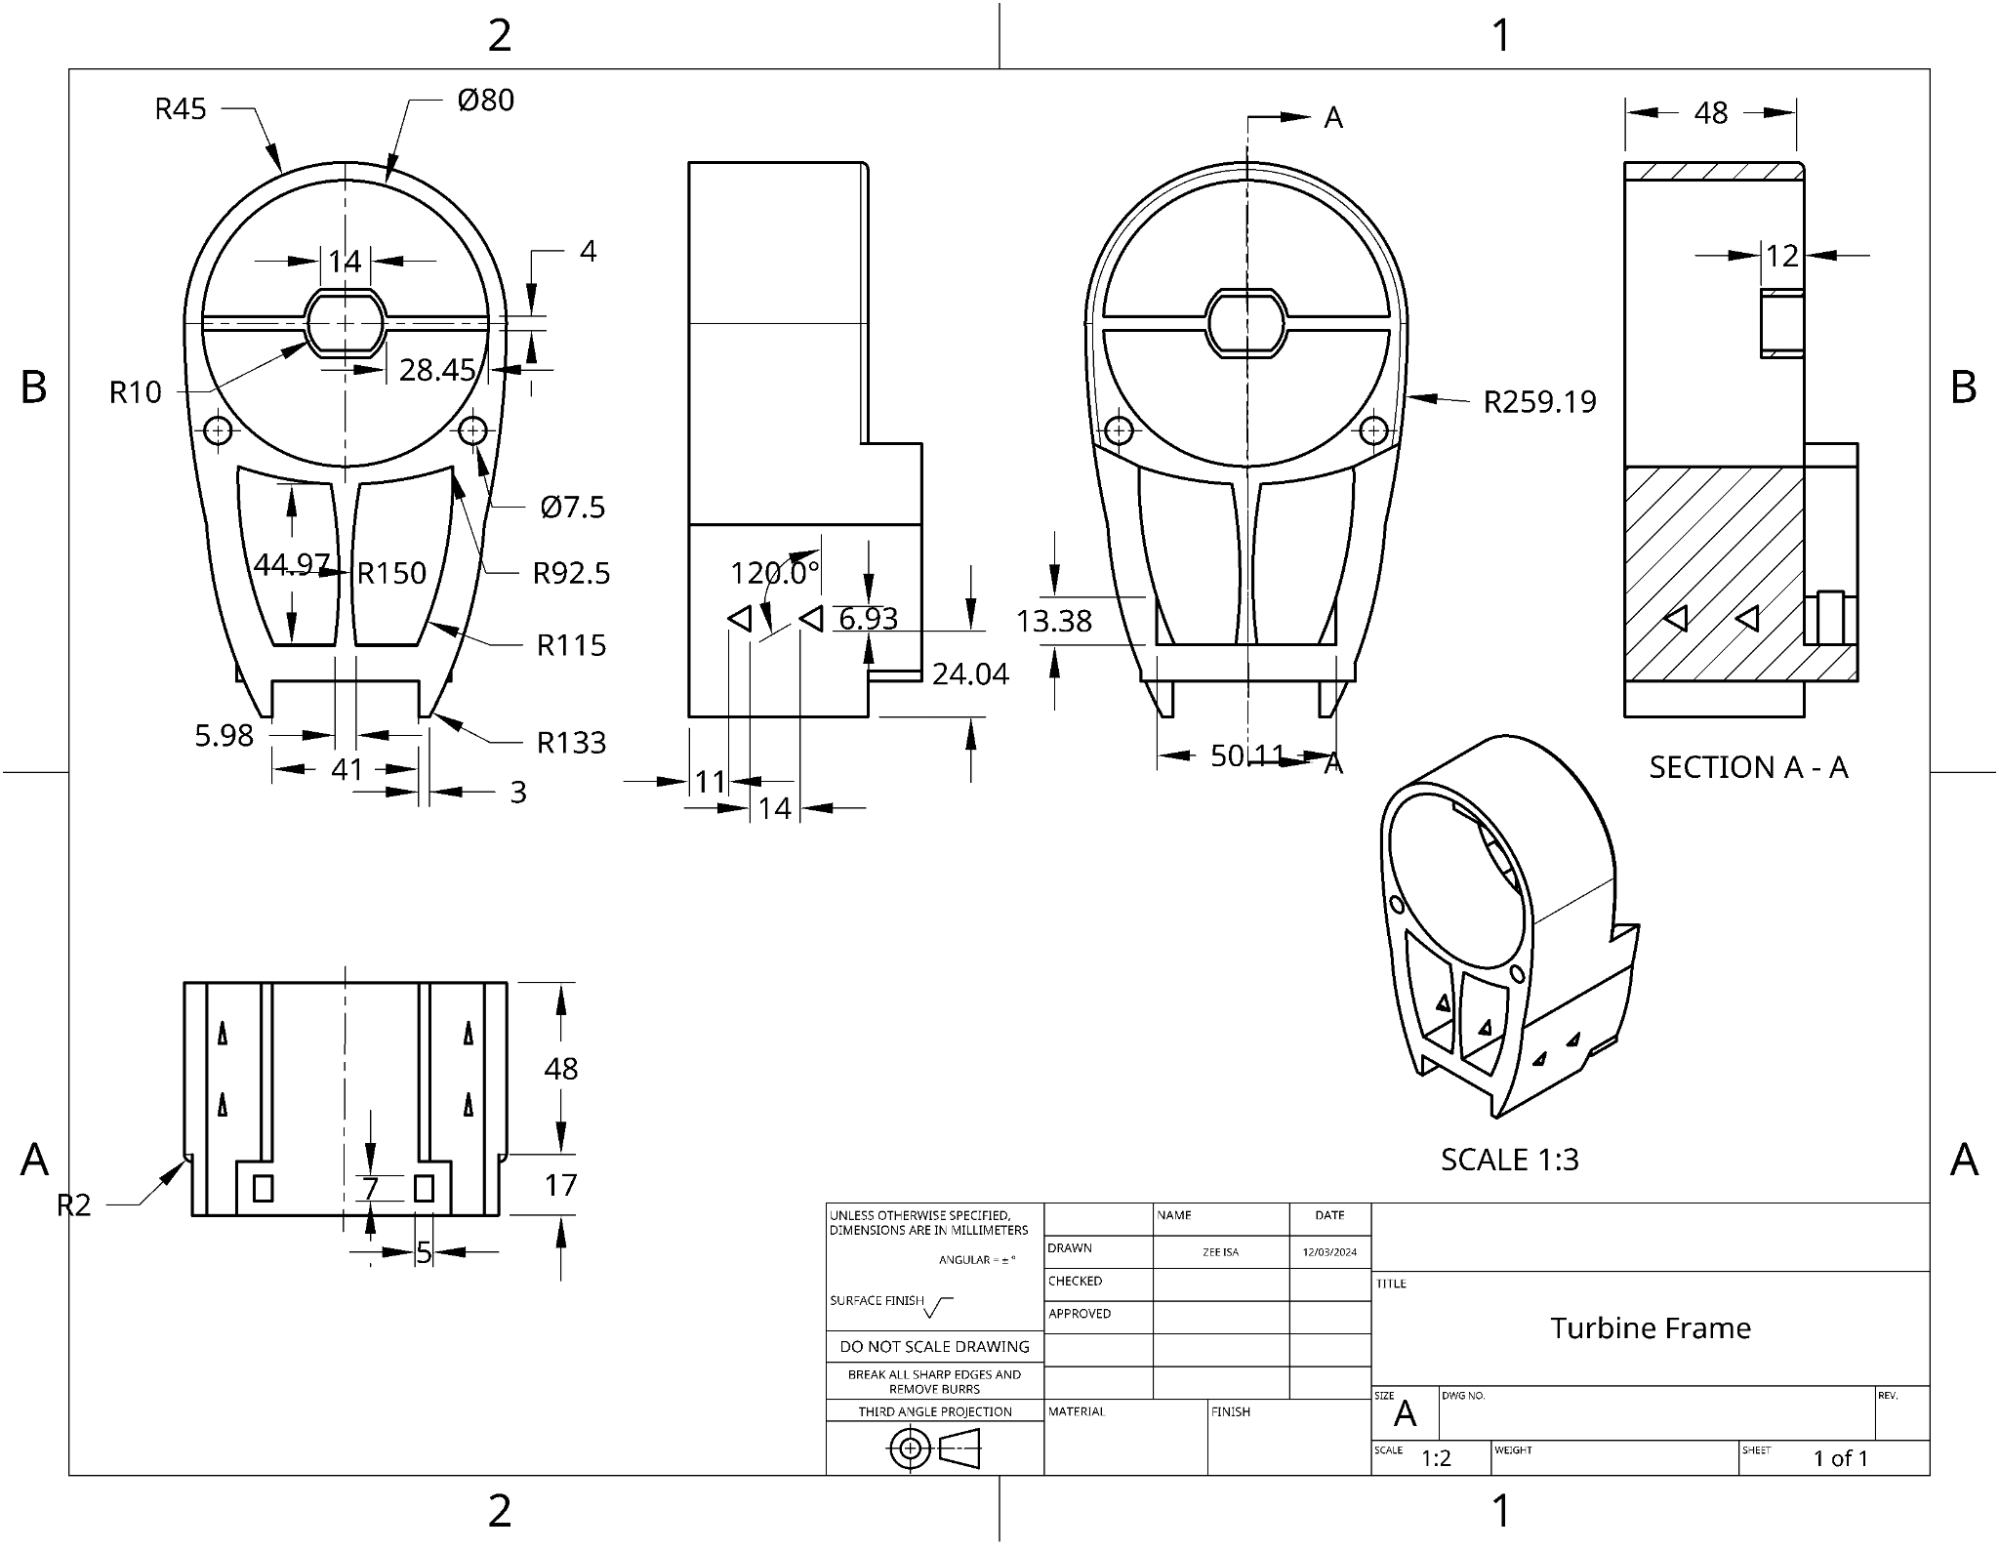
\includegraphics[width=1\linewidth]{Figures/TechTurbine}
			\caption[Turbine Tech. Drawing]{Technical drawing of the turbine frame.}
			\label{fig:techturbine}
		\end{figure}
			Attached to the inlet and processor, the turbine pokes above the sediment and uses a fan blade attached to a DC motor to measure the speed of the water. This motor is unpowered, and thus the voltage produced by its turning can be measured and converted to the speed of the water. This information about the flow rate is necessary to calculate how long it will take particles passing by the processor to arrive at the selector, and thus to determine when the selector should flip if a microplastic is detected. To aid in this, a bearing is used to ensure that the turbine blades are aligned and rotate smoothly, and a small attachment is used to interface the bearing with the frame. 
		\begin{figure}[h]
			\centering
			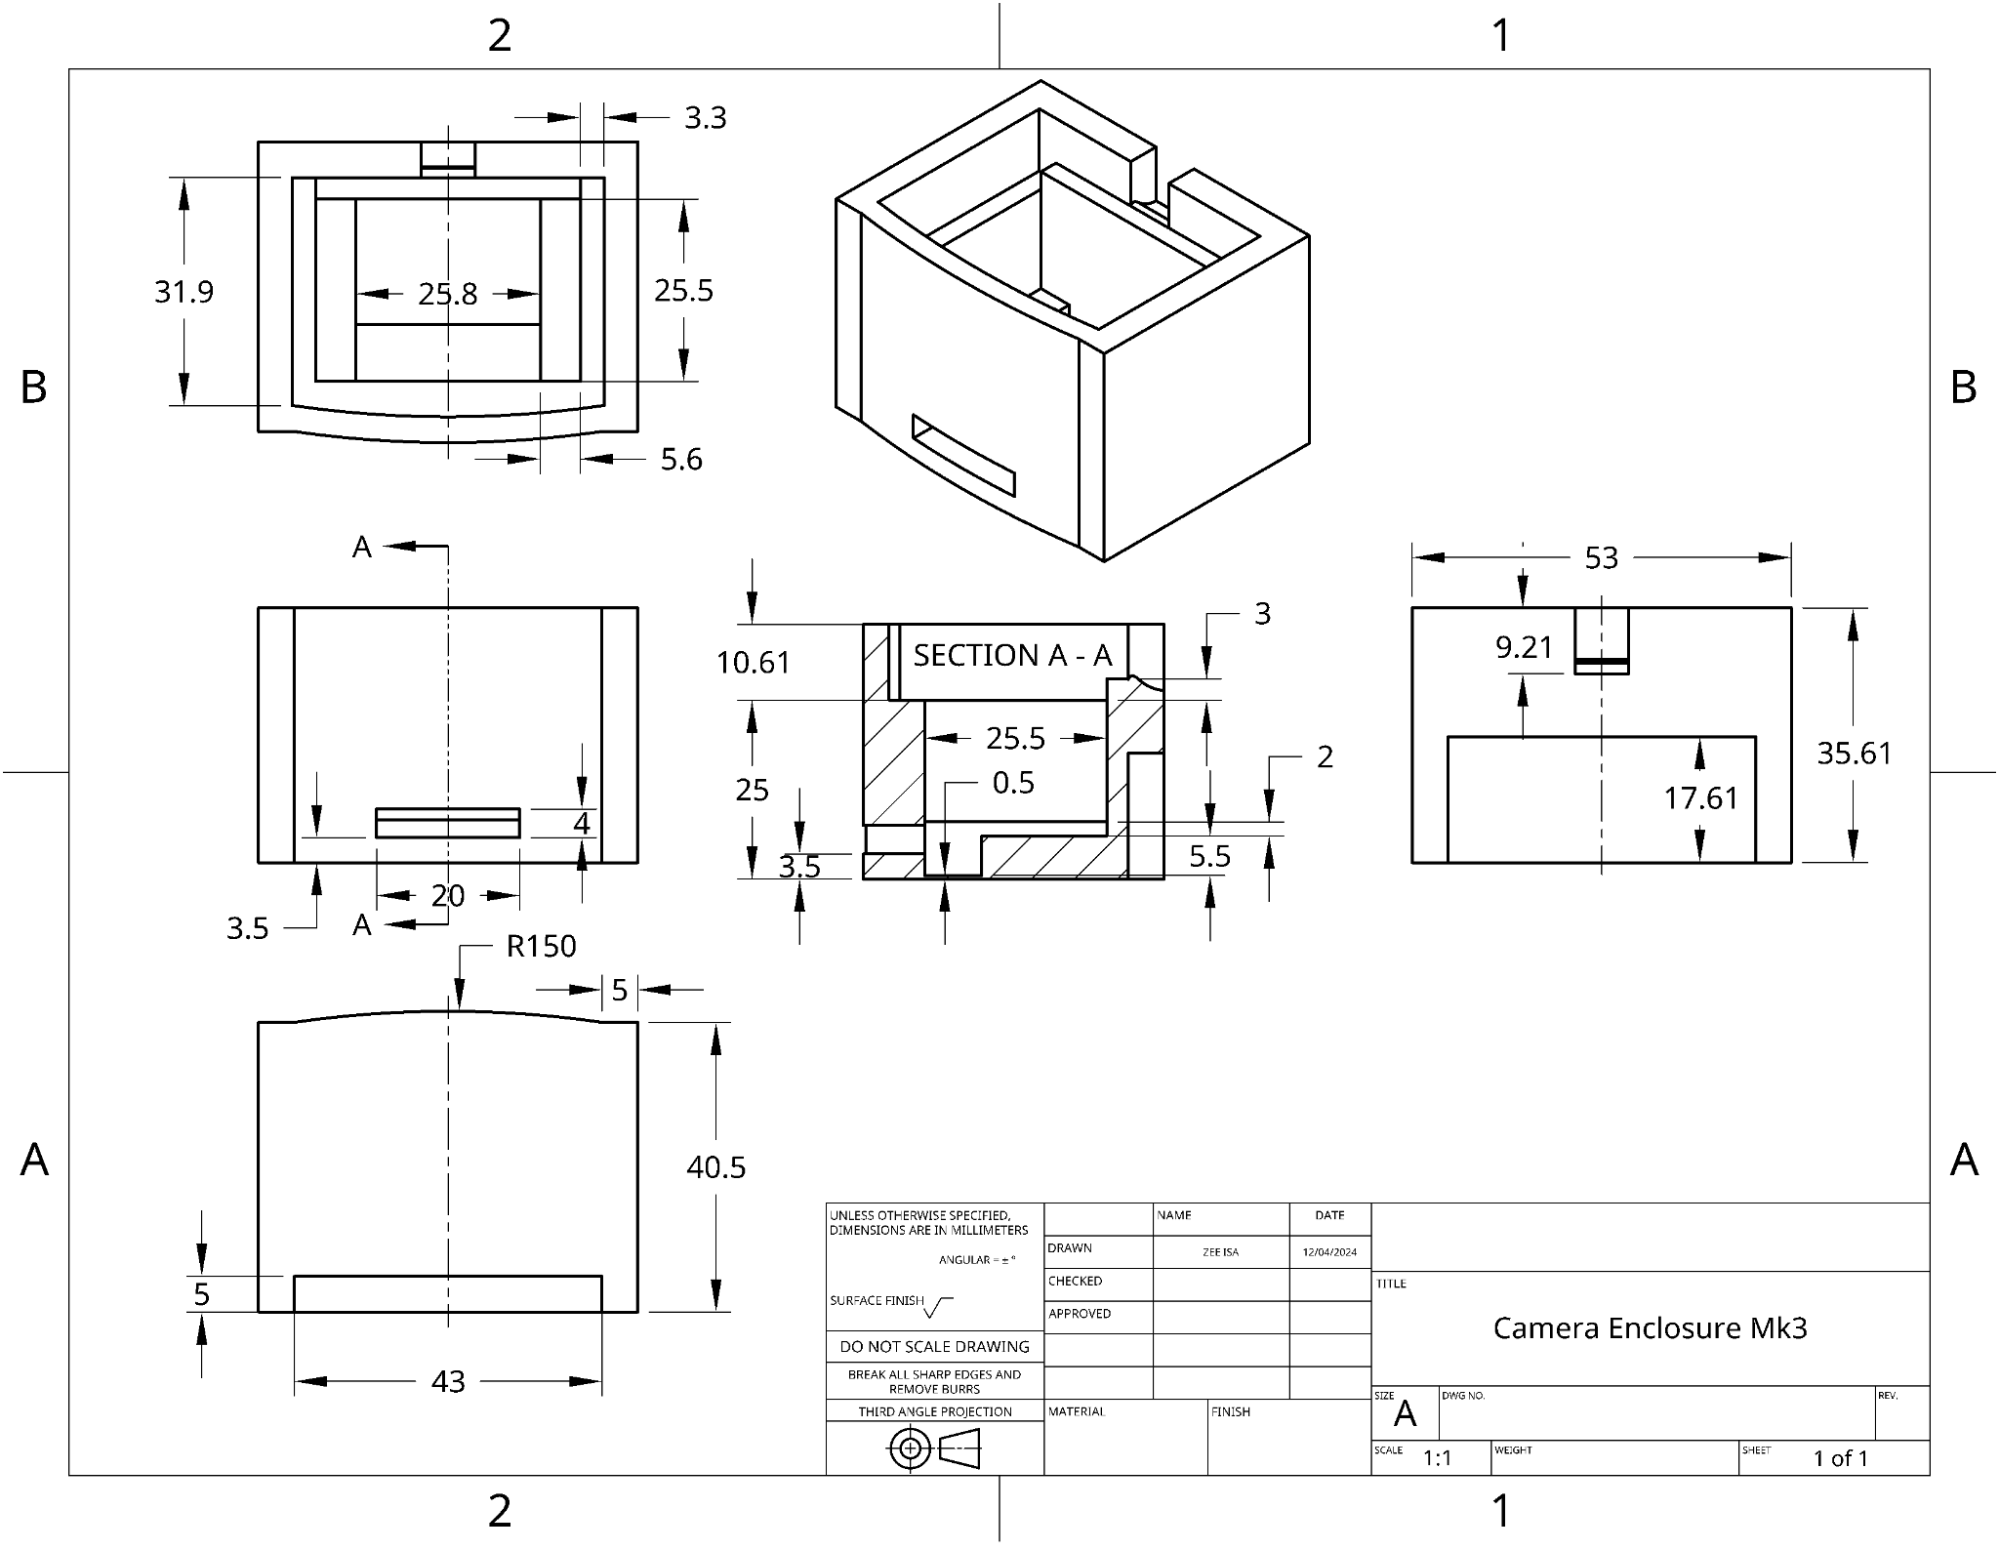
\includegraphics[width=1\linewidth]{Figures/TechCamBox}
			\caption[Camera Box Tech. Drawing]{Technical drawing of the camera enclosures.}
			\label{fig:techCamBox}
		\end{figure}
			On each side of the processor, there are also enclosures for the Raspberry Pi Cameras, with each enclosure waterproofed using 2-part epoxy. 
			\linebreak
			Next, the spine piece attaches to the intake and processor (eventually to the outlet and servo container as well) in order to connect each and ensure that the device retains rigidity without flexing under the pressures of the riverine environment. Throughout the spine, there are holes for pins to pass through which connect to the other components, and the spine provides a centralized support and method of connection which doesn’t rely on glue, epoxy, or fasteners. 
			\begin{figure}[h]
				\centering
				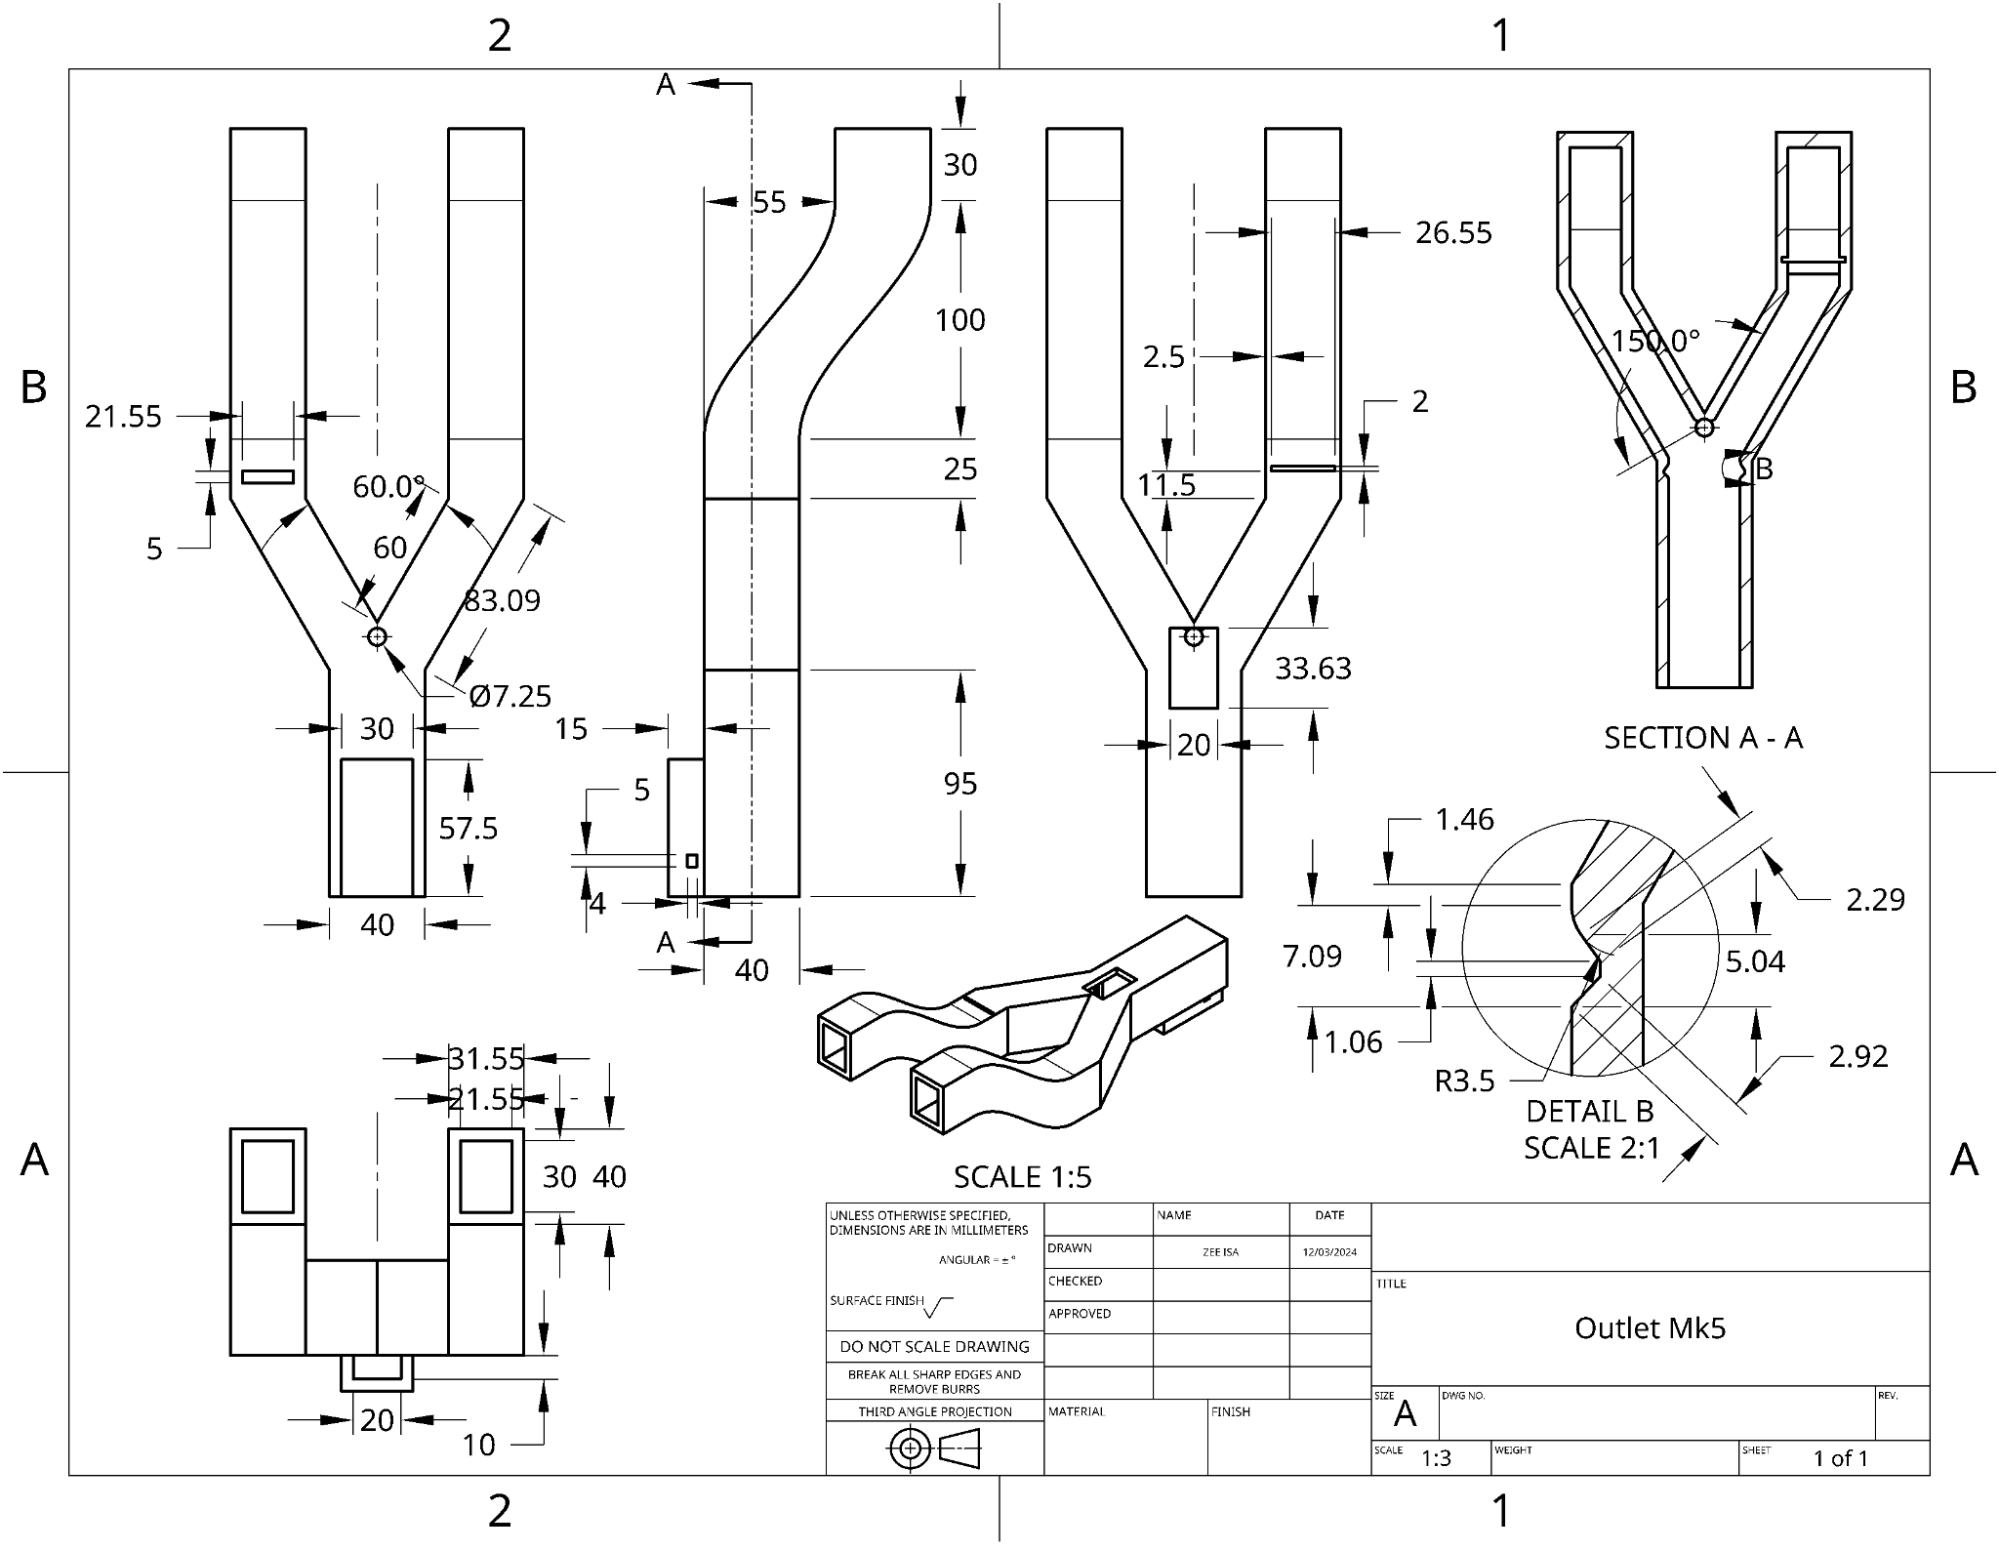
\includegraphics[width=1\linewidth]{Figures/TechOutlet}
				\caption[Outlet Tech. Drawing]{Technical drawing of the outlet.}
				\label{fig:techOutlet}
			\end{figure}

			The next part attached to the spine is the outlet, which completes the path of particle travel through the device, splitting into two portions and comprising the selection portion of the device. There are three primary features of the outlet which enable this selection functionality, and these are: 
		\begin{enumerate}
			\item Grooves which fit closely with the selector,
			\item A slot for placement of a filter,
			\item And a hole through which the selector interfaces with the servo.
		\end{enumerate}
		Note as well the rectangular hole in the top of the outlet piece, which is later plugged by the outlet cover. This hole exists as a human-necessary piece to allow the selection flipper to be placed inside of the outlet piece manually, as otherwise it would be very difficult to do so.			
		\begin{figure}[h]
			\centering
			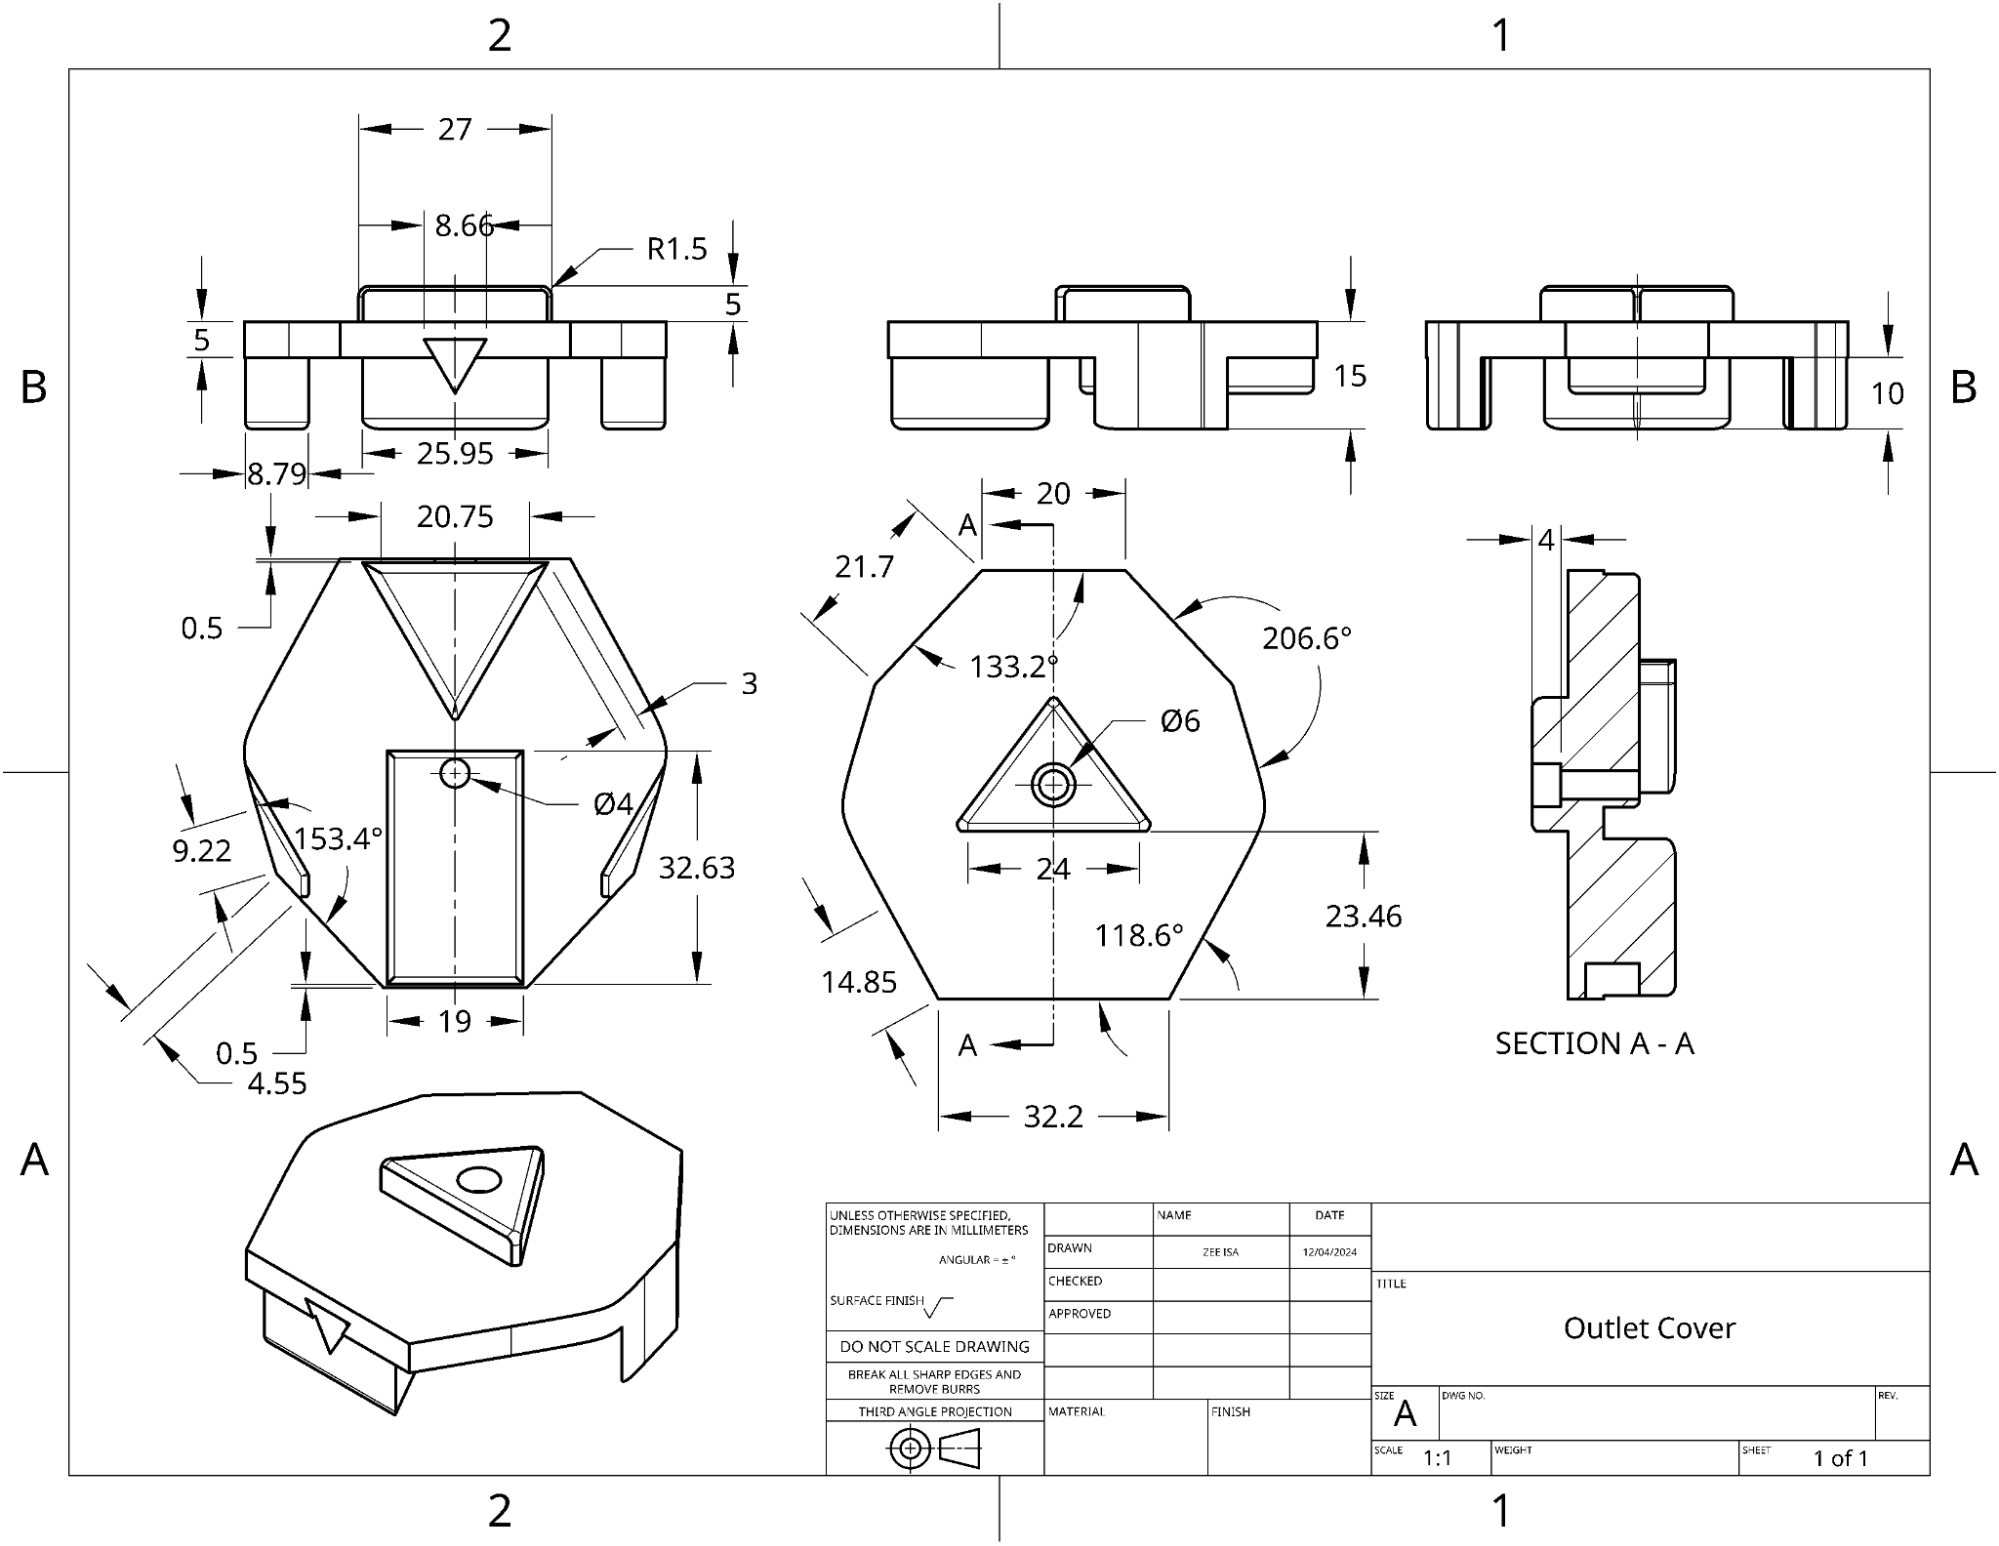
\includegraphics[width=1\linewidth]{Figures/TechCover}
			\caption[Outlet Covering Tech. Drawing]{Technical drawing of the covering over the outlet's top hole.}
			\label{fig:techCover}
		\end{figure} 
		Regarding the flipper, it, along with its supporting axle and servo connection, comprises one of the most important parts of the project. As seen in figure \ref{fig:techFlipper}, the flipper has three primary features: first, the square slot at the bottom of the part interfaces with the rotating servo, next, the circular hole at the top allows an axle which keeps the flipper aligned, and finally the flat surface of the flipper itself. 
		\begin{figure}[h]
			\centering
			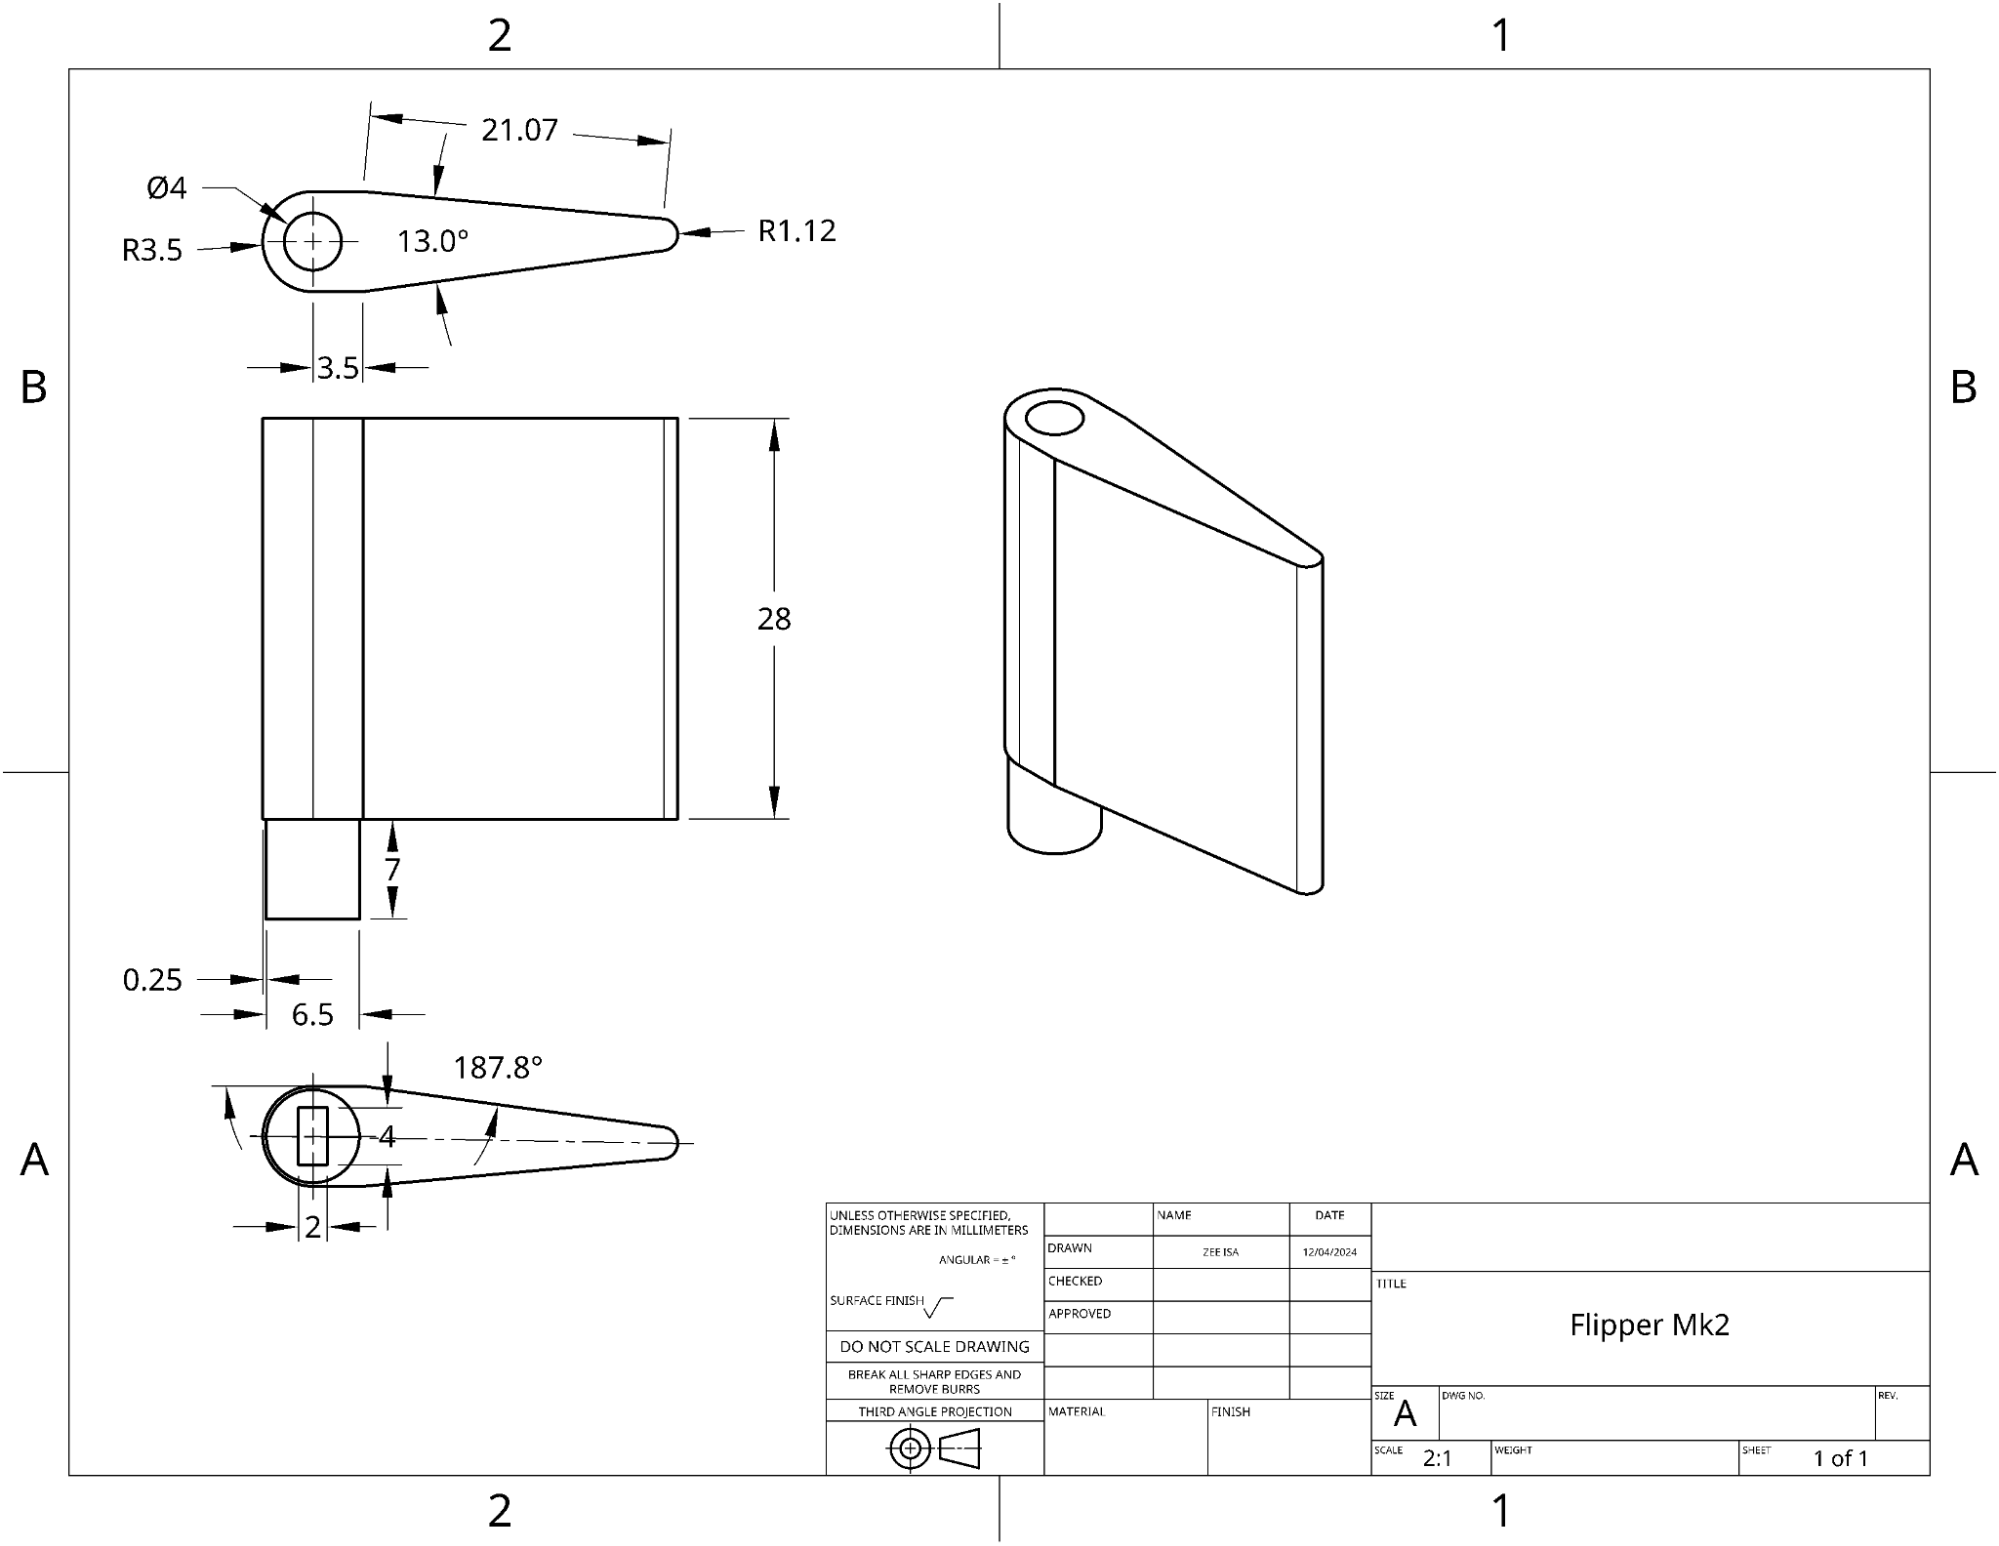
\includegraphics[width=1\linewidth]{Figures/TechFlipper}
			\caption[Flipper Tech. Drawing]{Technical drawing of the flipper.}
			\label{fig:techFlipper}
		\end{figure} 
		The servo itself is contained within a covering which protects it from impact and significant foreign particle entry, though this covering is not intended to be completely impermeable for water as the servo is IP68 rated (able to be continuously submerged in up to 3 meters of water). This covering also serves the purpose of aligning the servo with the flipper very precisely, as the flipper and its attachment points are all only a few millimeters in size. 
		\begin{figure}[h]
			\centering
			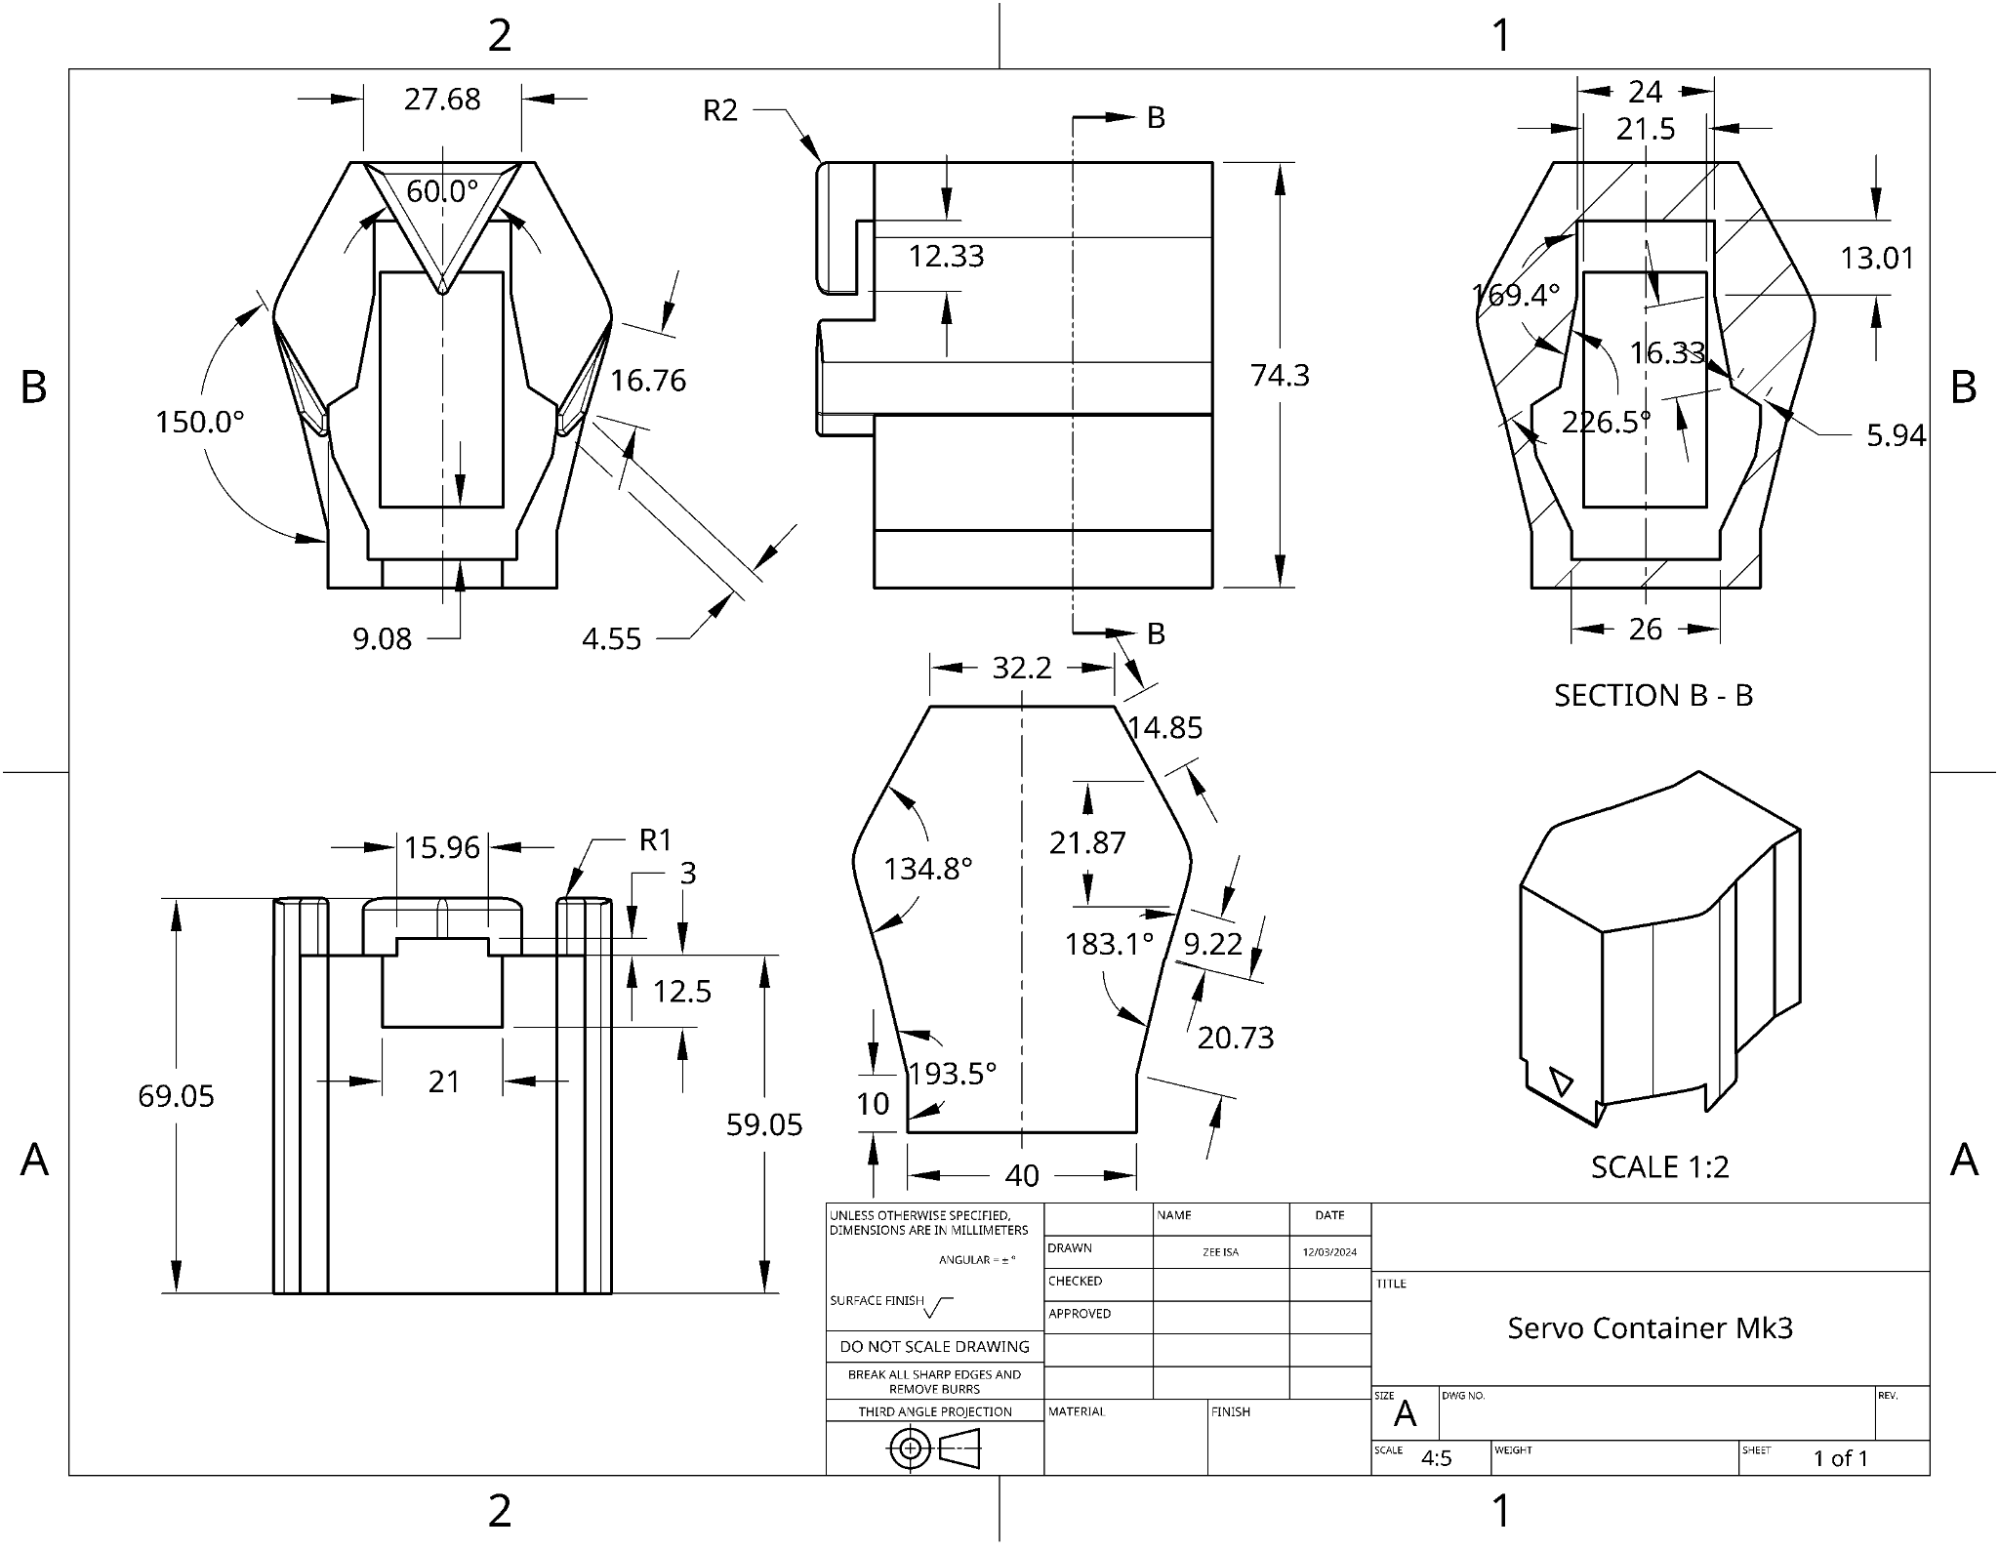
\includegraphics[width=1\linewidth]{Figures/TechServoBox}
			\caption[Servo Container Tech. Drawing]{Technical drawing of the servo containment box.}
			\label{fig:techServo}
		\end{figure} 
		These pieces comprise the majority of the aforementioned path through the device which microplastics and other particles take, but a few other pieces are also critical to the device’s functioning. The most important of these is the compute module holder, a piece designed to be totally impermeable to water as expanded upon in section \ref{sec:programmingArch}. 
		
		
	\subsubsection{Programming Architecture}\label{sec:programmingArch}
	\begin{figure}[h]
		\centering
		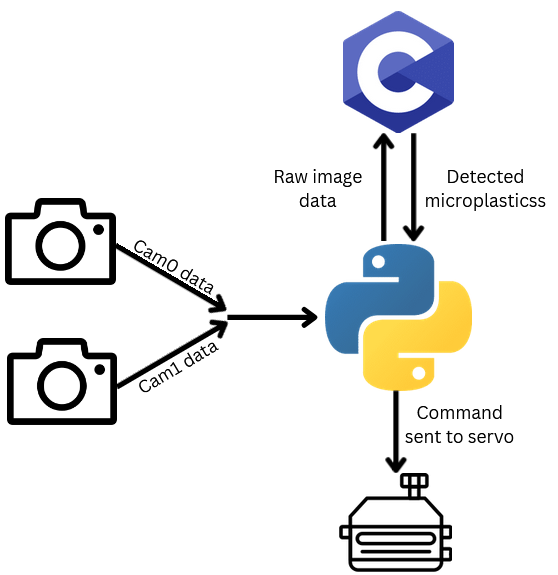
\includegraphics[width=1\linewidth]{Figures/ProgrammingArch}
		\caption[Programming Architecture Diagram]{Diagram of the device's programming architecture.}
		\label{fig:ProgArch}
	\end{figure} 
		The programming of the device described here is relatively simple, with two modules (one in C, one in Python), interfacing with the camera data provided by the onboard RPICam-V2s. The python module acts as the primary “master” program which collects the data from the cameras, sends it to the C program as a 3D array containing each image’s pixels and their colors, receives the processed data, and sends a command to the servo. The servo commands are handled by storing the next command and its timestamp, then sending the command to the servo once the timestamp is reached. This timestamp is determined via an interaction with the turbine attached to the device which provides a voltage by turning a small dc motor. This voltage can be read by the Raspberry PI, then using a reference table comparing external water speed to internal water speed (obtained by interpolating values from a simple CFD simulation), the time from detection to selection can be determined. The primary difficulty with accomplishing these aforementioned processes and the reason why C must be used instead of doing all processing in Python is that all actions must be performed within 4000 $\mu$s (0.004 seconds), a time span which is simply too short for a language as slow as Python. 
	
	\subsubsection{Electrical Design}
	\begin{figure}[h]
		\centering
		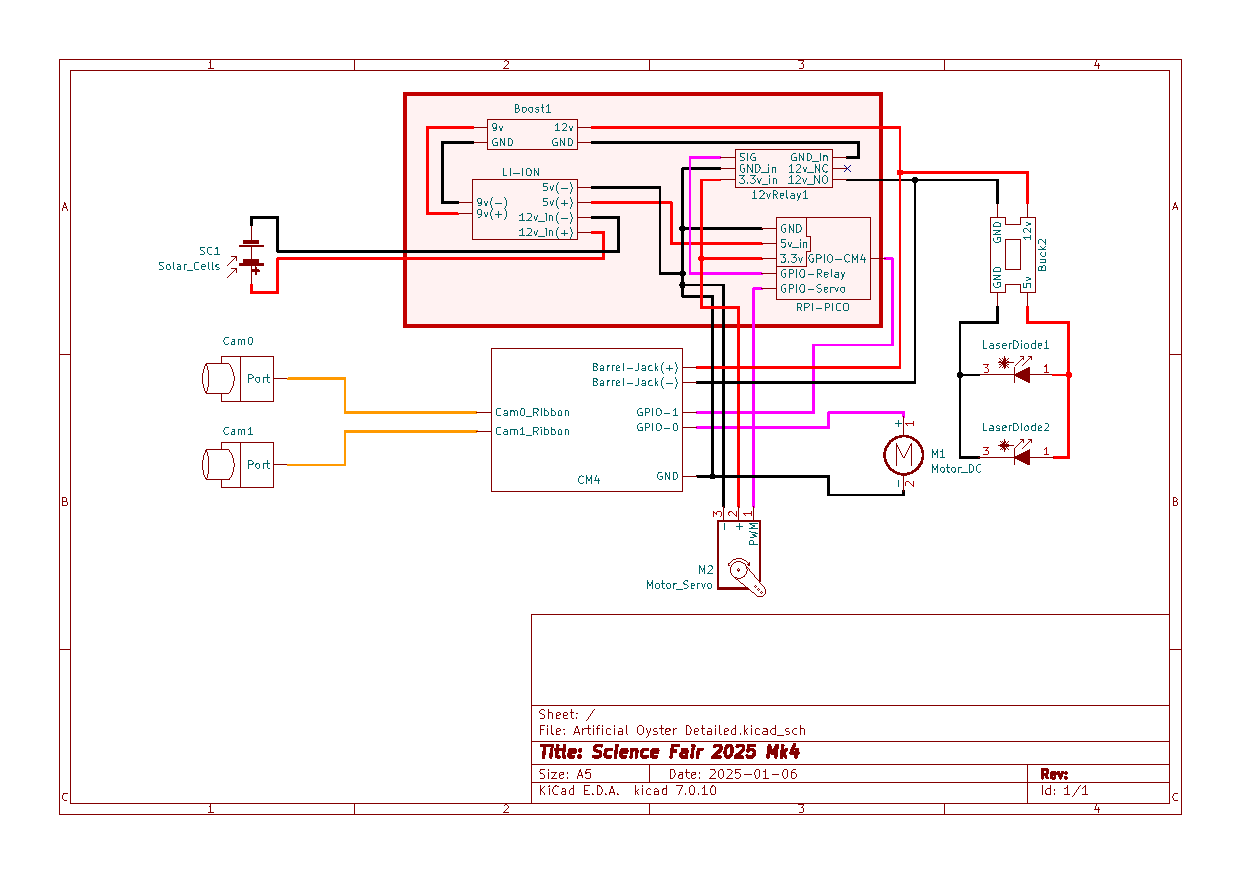
\includegraphics[width=1\linewidth]{Figures/ElecSchematic}
		\caption[Electrical Schematic]{The device's electrical schematic with several elements simplified for comprehensibility, most notably with the Raspberry Pi Compute Module 4 and its I/O board condensed to just 7 inputs/outputs.}
		\label{fig:ElecSchem}
	\end{figure}
	
	Due to the very high cycle speeds required by the device and relatively simple electrical requirements, the electrical schematic is relatively simple. In this diagram, the Raspberry Pi CM4 and I/O board are greatly simplified to only include the inputs and outputs which are actually used within the device. One interesting aspect of the device is shown in the upper section of the electrical schematic, where a Raspberry Pi Pico 1 is used to regulate power to the RPI CM4. This method is used primarily due to a quirk of the CM4’s camera management systems which causes the second camera (counter-intuitively using the cam0 port on the I/O board) to be disconnected from the RPI if the device is rebooted using standard methods. This is likely because the camera management libraries used for the RPI were not intended to operate two cameras at once, however, the issue can be circumvented simply by powering off the RPI abruptly instead of rebooting or powering off in a standard way. This requirement means that some external device must be responsible for controlling power supplied to the CM4, and as shown, a Raspberry Pi Pico fulfills this role by controlling a 12v solid state relay. This also simplifies time and voltage based operation to ensure that the device’s batteries never lose too much voltage, allowing operating times to change dynamically depending on the weather (sunlight) on any given day. 
	\paragraph*{Power Generation}
	
	\begin{figure}[h]
		\centering
		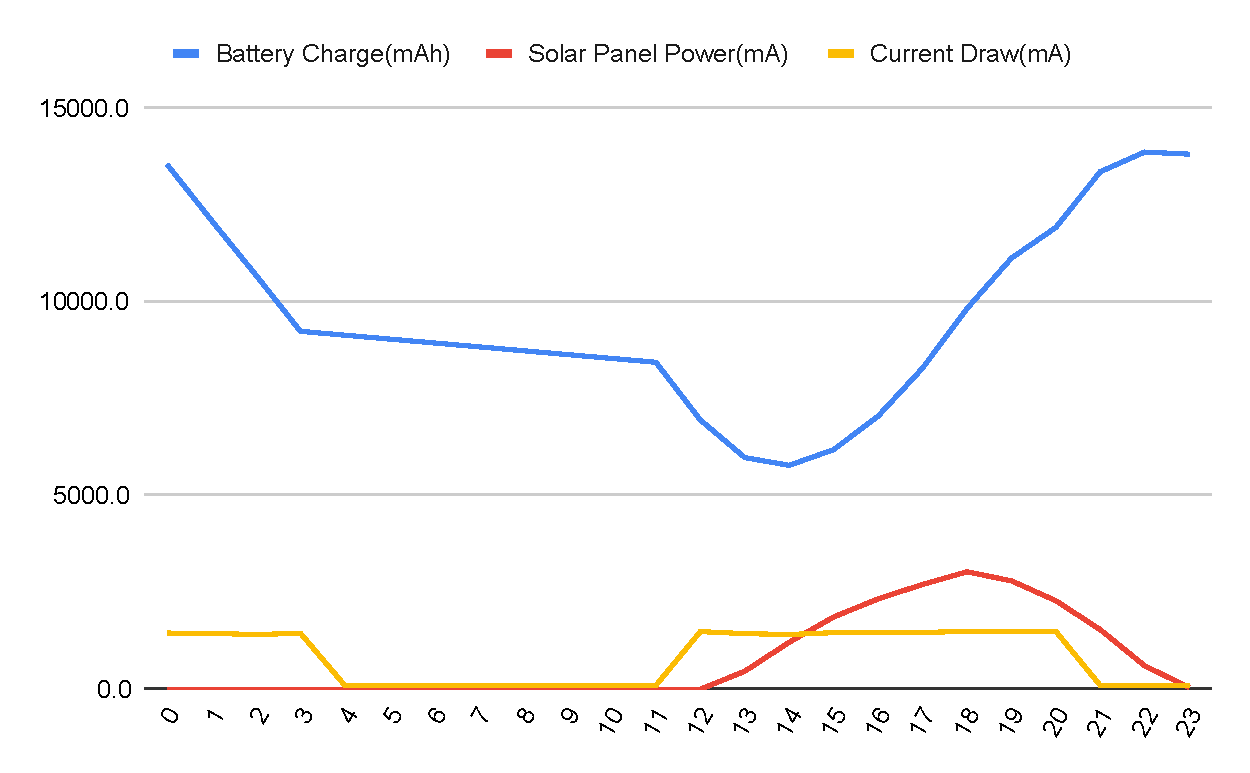
\includegraphics[width=1\linewidth]{Figures/MedDay}
		\caption[Power Consumption Graph]{Graph of the device's power metrics over the course of one average day in Milwaukee, Wisconsin.}
		\label{fig:ElecMod}
	\end{figure} 
	
	\begin{figure}[h]
		\centering
		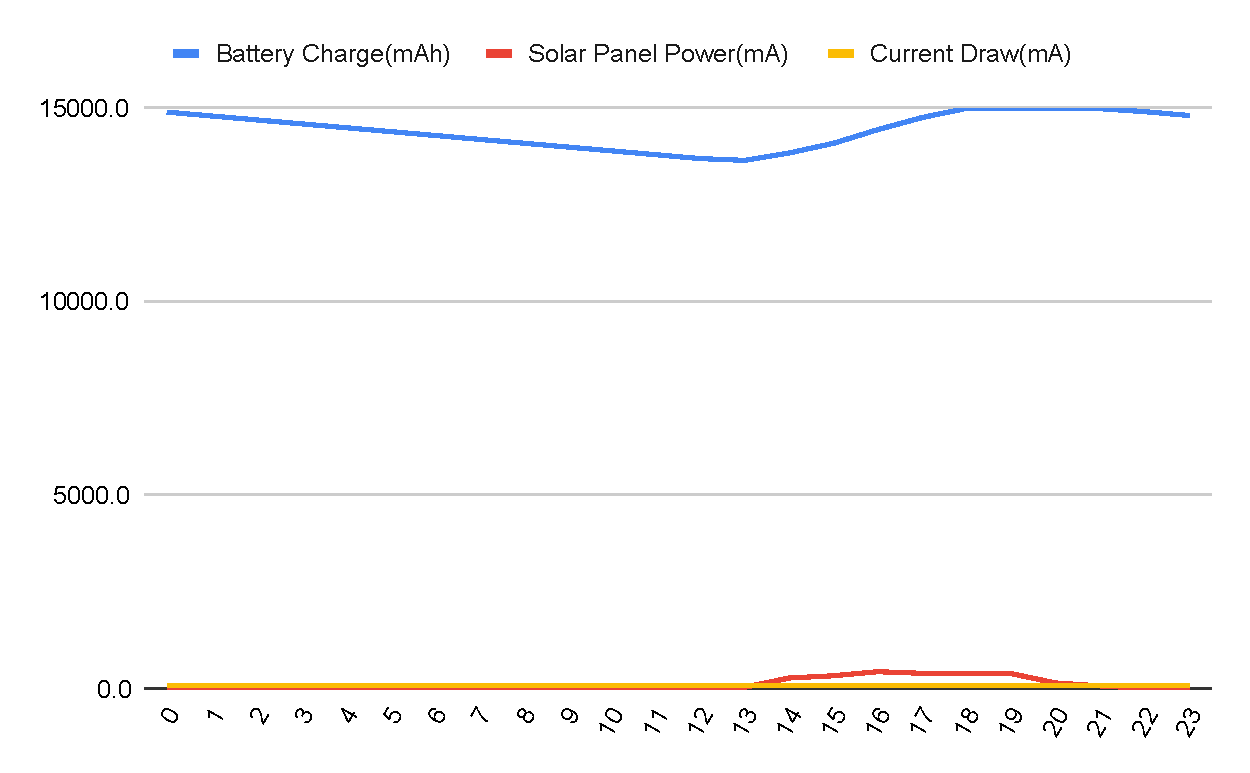
\includegraphics[width=1\linewidth]{Figures/LowDay}
		\caption[Power Consumption Graph]{Graph of the device's power metrics over the course of one day in the bottom 10\% of GHI in Milwaukee, Wisconsin.}
		\label{fig:botPowerGen}
	\end{figure} 
	
		\begin{figure}[h]
		\centering
		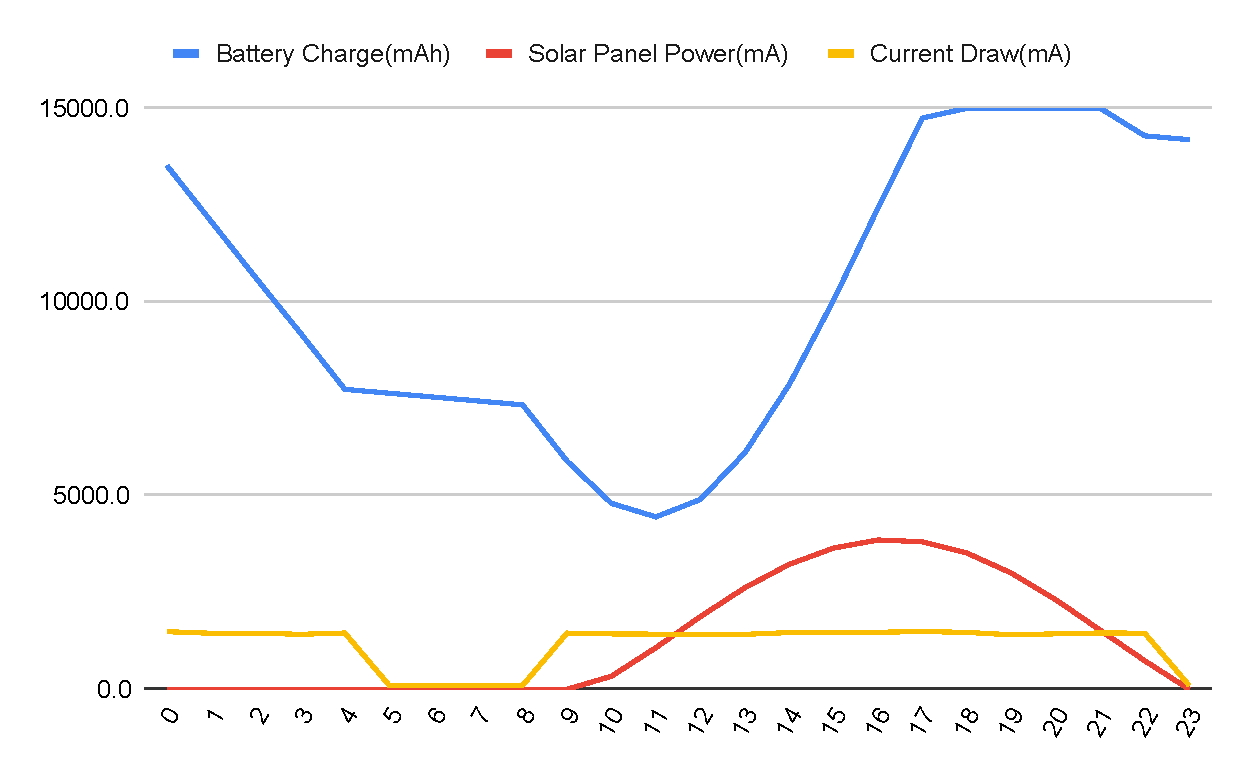
\includegraphics[width=1\linewidth]{Figures/HiDay}
		\caption[Power Consumption Graph]{Graph of the device's power metrics over the course of one day in the top 10\% of GHI in Milwaukee, Wisconsin.}
		\label{fig:topPowerGen}
	\end{figure} 
	Several different power generation techniques were considered for this device, with hydropower and solar being the two primary contenders. After evaluation, solar was selected for this project due primarily to:
	\begin{enumerate}
		\item The testing location
		\begin{itemize}
			\item The lower Milwaukee River's water isn't deep enough, and doesn't flow fast enough, for significant hydroelectric power generation
			\item The specific testing location has several small and bare islands within a few meters of the location
		\end{itemize}
		\item Power requirements
			\begin{itemize}
				\item The device simply consumes too much power for a reasonably sized complementary hydroelectric installation to power it
			\end{itemize}
		\item Cost
		\begin{itemize}
			\item Solar panels are much cheaper than a similar output hydroelectric generator if COTS parts are used
		\end{itemize}
	\end{enumerate}
	
	The graph shown in figure \ref{fig:ElecMod} shows how the device’s battery charge, power input, and current draw would fluctuate on an average day in Milwaukee, Wisconsin (the location of testing). As shown, the battery charge never drops below 25.4\%\textemdash ensuring that sufficient voltage is maintained throughout the day. In this model, the device operates for 13 hours, thus filtering roughly 51.5 m3 of water as derived from figure \ref{fig:riverCrosssec}.  
	
	
	\subsubsection{Waterproofing}
	For the final device to be successful, there are three parts that must be prevented from ever contacting water directly\textemdash those being the RPI compute module and the two cameras on either side of the processor. If any of these components contact the water then corrosion will soon follow, greatly reducing the device’s lifespan. Waterproofing is accomplished with a combination of multi-layered walls, small exits, and coating with 2-part epoxy to ensure that no water ever enters. One other approach of lifting the compute module above the water was considered, however, this would conflict with tenet \# 1 of Design Principles, subsection \ref{subsec:TechDesign}\textemdash if the compute module were raised above the water then it would present an obstacle to humans and compromise the environmental services provided by the river. 
	
	\section{Testing}
	\subsection{River Impact Testing}
	Testing for the device will begin with a thorough analysis of the inadvertent impacts which the proposed device could have on riverine ecosystems due to its constant irradiation of water flowing through the processor. This irradiation is momentary, and will likely have a minimal effect on life within any river which the device operates inside of\textemdash but given that in a typical river (the Milwaukee River being used here as “typical”) the device could process massive quantities of water each day. This quantity of water processed can be approximated by multiplying the cross-sectional area of the device’s inlet by the flow rate of the river\textemdash something which can be approximated by comparing the river’s discharge with the overall river’s cross-sectional area. The calculations to find this value are as follows:
	\begin{enumerate}
		\item Using data retrieved from USGS’ Upper Midwest Water Science Center in Milwaukee (figure \ref{fig:riverCrosssec}), the cross-sectional area of the river near the site of testing can be calculated to be roughly 127 ft$^2$
		\item Using more USGS data, we find the total river discharge = 423 ft$^3$/s 
		\item Find approximate depth of river using figure \ref{fig:riverCrosssec} 
		
		\begin{itemize}
			\item 1.2 ft 
		\end{itemize}
		
		\item Use satellite imagery of location with depth to find rough cross-sectional area of river in the area of testing 
		\begin{itemize}
			\item 1.2 ft average depth * 106 ft wide =  $\approx$127 ft$^2$ cross-sectional area
		\end{itemize}
		\item Divide total discharge (423 ft$^3$/s) by cross sectional area 
		
		 423 ft$^3$s / 106 ft$^2$ = 3.99 ft$^3$/ft$^2$/s
		
		\begin{itemize}
			\item This unit measures the volume of water passing through a 1’x1’ area perpendicular to the shore in one second. 
		\end{itemize}
		\item Multiply this by the total area of the device’s opening - 0.01 ft$^2$ $\times$ 3.99 ft$^3$/ft$^2$/s = 0.04 ft$^3$/s
		\item At this point we convert this value to the metric system for the sake of simplicity 
		
		\begin{itemize}
			\item $0.04 ft^3/s \rightarrow 0.0011 m^3/s$
		\end{itemize}
		
		\item 0.0011m$^3$/s * 86,400 s/day $\approx$ 95 m$^3$/day of water
		
		\item Multiply total water flowing through the device in one day by the fraction of the day for which the device operates
		
		\begin{itemize}
			\item $95m^3/s \times 13/24 = 51.5m^3$
		\end{itemize}
		
	\end{enumerate}
		\begin{figure}[h]
		\centering
		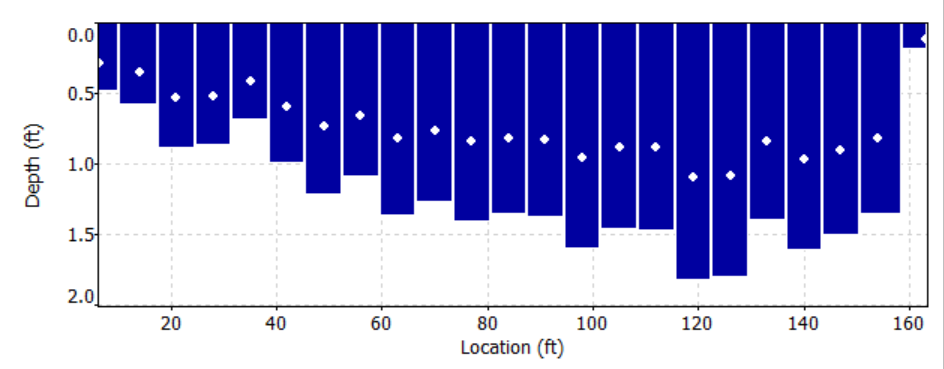
\includegraphics[width=1\linewidth]{Figures/RiverCrosssection}
		\caption[River Cross Section]{A cross section of the Milwaukee River at USGS' gage height station, very near the location of testing for this project.}
		\label{fig:riverCrosssec}
	\end{figure}
	
	Given this large quantity, and given that benthic water is far more biodiverse than pelagic waters, it is critical that the device proposed here does not cause undue harm to microorganisms. Due, again, to the high biodiversity of benthic regions, it is very difficult to predict the impacts which this could have on any single ecosystem without testing real samples\textemdash thus to ensure that the testing conducted here does not have significant unintended consequences on the environment, an examination of these impacts must be conducted. 
	
	\subsubsection{Procedure}
	The testing conducted here will be relatively simple\textemdash the goal is simply to assess whether or not short-term exposure to the laser light has a significant impact on microorganisms within Milwaukee River Water. To accomplish this, multiple samples of the water and detritus from the benthic region will be taken\textemdash some from undisturbed flow and some with benthic sediment agitated upstream of it to ensure that significant quantities of benthic sediment are sampled. The samples will then be mixed together into a single, larger sample. After agitation, water will be collected using a pipette and broken into 20, 10mL portions which will be transferred into separate containers. 
	Next, each of these will be numbered 0-9 (2 samples per number) and irradiated via a short exposure to light from the lasers used within the processor. Each sample will be irradiated N times according to its label, (i.e. sample \# 4 will receive 4 short exposures to the laser light) simulating increasing levels of irradiation to compensate for uncertainties with the exact speed at which water will flow through the device. To ensure consistency with irradiation exposure times among the samples, a motorized gantry (the type found on a 3D printer) with a laser attached to it will be used to sweep over each sample with laser light.
	
	\begin{table}[h]
		\begin{tabular}{|l|l|l|l|l|l|}
			\hline
			Sample \#         & 0 & 1    & 2   & ... & 9    \\ \hline
			Exposure time (s) & 0 & 0.15 & 0.3 & ... & 1.35 \\ \hline
		\end{tabular}
		\caption[Laser Exposure Time Table]{Table of laser exposure times for each water sample. Note that in addition to the benthic water tests, simultaneous tests were conducted for surface water and water mixed directly with benthic sediment. Results were the same for each test.}
	\end{table}
	
	After all rounds of irradiation, each sample will be examined under a standard classroom microscope and the impacts of the irradiation will be qualitatively examined\textemdash checking primarily for microorganisms and other signs of life or lack thereof. For the tests to be considered satisfactory (i.e., for the existing laser to be used as opposed to a lower-power variant which would have less impact on microorganisms), all samples \# 1-3 should be essentially indistinguishable from the control sample. This range is chosen because given the flow rate of the Milwaukee River ($\approx$2 m/s) compared to the motorized gantry’s speed of 200mm/s, sample \# 1 will have been irradiated for roughly 10x longer than the river water traveling through the device will be exposed (sample \# 2 roughly 20x, \# 3 30x, etc.). If successful, this will remove any doubt that the device will have significant negative impacts on the river\textemdash although it is also important to note that this testing should be conducted every time that the device is placed in a new river to ensure that the local flora and fauna are not disturbed. It should also be noted that different times of year may have different active organisms, and thus more extensive testing ought to be conducted for long-term deployment.
 
	\subsubsection{Prediction}
	Given the results from several previous studies\footnote{Unfortunately, very little work has been done regarding the impacts of blue laser light exposure on microorganisms, even less on riverine microorganisms, and essentially none on exposures at the $<$1 second timescale. This is certainly an area for future research, however, given the minimal impacts found at times as high as several hours in the studies at the footnote, it can be inferred that similarly minimal impacts result from the singular $<$0.01 second exposure used here. As a result of the aforementioned lack of work on this topic, the cited studies are each only marginally related to the topic of interest here. } \cite{Dai_Gupta_Murray_Vrahas_Tegos_Hamblin_2012} \cite{lightExposure} \cite{Gorai_Katayama_Obata_Murata_Taguchi_2014} \cite{lightExposure2},  it is predicted that the brief laser exposure used in this project will have no detectable impact on microorganism populations. Combined with the incredibly low chance that any single organism passes through the device more than once, the lasers' overall impact on river health will be minimal.
	\subsubsection{Results}
		Samples were collected on November 10th, 2024 in the portion of the Milwaukee directly behind the Nicolet High School Forest on 6701 N Jean Nicolet Road. On the day of collection, the weather was relatively clear and roughly 13° C. Roughly 3-4 mm of rain occurred prior to testing—this was determined to be insufficient to justify rescheduling sample collection. To evaluate the samples, the above procedure was carried out and each sample was examined with a microscope roughly 1 hour later on the day of collection. 
	Results, as hypothesized, indicated that the irradiation had very little effect on the microorganisms within the samples. After qualitative analysis, no appreciable differences could be detected between any of the samples—a reasonable result given that no sample was exposed for more than 1.35 seconds in total. To further confirm the result, the lasers were manually swept over the 9-exposure samples several more times, and even after seconds of exposure neither the number of moving microorganisms nor the appearance of any other plant matter changed noticeably. 
	The next logical step is examining the impact of the lasers on the benthic microbiome—something which was not done in this study due to the risks associated with culturing unknown bacteria outside of a lab. It is very likely that, consistent with predictions, even more extensive irradiation would have a limited impact on river microorganisms or bacteria. 
	
	\subsection{Empirical Testing}
	\subsubsection{Procedure}
	The final portion of testing involves using the device in its real-life operating conditions in order to evaluate its real performance over an extended period of time—in this case for 24 hours. To do this, several steps will be taken: 
	\begin{enumerate}
		
		\item Set up control measurement:	
		\begin{enumerate}
			\item On the end of the outlet which doesn't filter water, a net with the same pore diameter as the device’s filter will be fixed in order to gather a complete sample of microplastics which pass through the device. This provides an approximation for how many microplastics ought to be filtered out by the device and will allow measurements to be made regardless of circumstances which could increase or decrease the quantity of plastics measured. For example, if testing takes place within a short period after precipitation, this control will adjust for the possible increase or decrease in benthic flow.
		\end{enumerate}
				
		\item Set up device:
		\begin{enumerate}
			\item In a section of the Milwaukee River roughly representative of the entire length, the device will be buried as shown in figure \ref{fig:InletInSitu}, then after setup of all systems and activation, the device will be left in-situ for the next 24 hours to simulate an entire day of operation. 
		\end{enumerate}
		
		\item Data analysis:
		\begin{enumerate}
			\item To analyze the data collected, the quantities of microplastics filtered by the nets on both sides of the device will be compared, and after counting the microplastics in each conclusions will be reached regarding: 
			\begin{enumerate}
				\item What percentage of the total benthic microplastic quantity is collected,
				
				\item How effectively the device avoids collecting non-microplastic material, and
				
				\item How well the device sustains its battery life, manages heat, etc.
				
			\end{enumerate}
		\end{enumerate}
		
	\end{enumerate}
	With this information collected, the device’s overall efficacy can be determined, and subsequent improvements or alterations can be made and re-tested.
	
	\paragraph*{Processing and Counting MPs}
	Processing the microplastics will follow the procedure used in \cite{LenakerEtAlvertdist}(derived from \cite{Zobkov_Esiukova_2016}), the steps to this procedure being:
	\begin{enumerate}
		\item Remove microplastics and other collected sestons from device and place into glass bowls 
		\item Use Fenton's reagent to dissolve  
		\item After organics have dissolved, use 4.5\% Hydrochloric acid to dissolve any calcites(shells)
		\item Wash and count by hand
	\end{enumerate}
	
	\subsubsection{Predictions}
	\label{subsubsec:predictions}
	The quantity of microplastics to be collected by the device can be simply approximated by using measurements from previous studies in tandem with data on total suspended solids (TSS) from USGS. Here, we find from \cite{LenakerEtAlvertdist} that microplastic concentrations near the intended testing site (the lower Milwaukee River) are approximately 2000 MP/kg, and additionally we find that this area's TSS measures roughly 22.1mg/L. Next, multiplying previous figures of total water filtration per day (51.5 m$^3$, 51500 liters) by TSS concentration (22.1mg/L), we find that the device will filter roughly 1.14kg of suspended solids. Multiplying this value by the concentration of microplastics per kilogram of sediment(2100MP/kg), we determine that the device should collect roughly 2400 microplastics over the duration of testing. Upper and lower bounds for this value can also be calculated using the extreme values ever measured on the Milwaukee River (2.1mg/L, 1400mg/L, \cite{USGSMil}, \cite{MKETSS}), arriving at 227 and 151,410 microplastics respectively. 
	\linebreak
	There are a few key assumptions which are necessary for this modeling to be accurate, those being:
	\begin{enumerate}
		\item The concentration of microplastics in the sediment must be relatively constant throughout the Milwaukee river (or at least must not fluctuate overly significantly to form hot spots of microplastics)
		\item The river must not flow more than $\approx$ 2 m/s
		\item The 2.5 cm top-sediment collected in \cite{LenakerEtAlvertdist} must be representative of the benthic flow's microplastic concentration
		\item There must be a positive correlation between TSS and suspended microplastics
	\end{enumerate}
	If these limited assumptions are correct, then it is likely that the device will operate as planned. Given this, a collection of roughly 2400 microplastics is predicted if tested for an entire day.
	
	This project's testing occured for a more limited period of 4 hours, as benthic sediment concentrations do not significantly fluctuate over time, and a more limited testing period simplifies several aspects of experimentation. In addition, the survivability of a benthic device primarily depends on water ingress protection\textemdash and with a successful 4 hour long test, the device will have passed the equivalent of 8 consecutive IP68 rating tests (the test which typically must be passed to qualify products as "waterproof"). Given this limited testing period, the predicted figure of 2400 MPs/day can be divided into 400 MPs/4 hours. This figure has upper and lower bounds at 25,235 and 38 MPs, respectively, assuming that TSS on the day of testing falls within previously measured maximum and minimum TSS values.
	\linebreak
	In addition to testing the device, a 500 mL water sample will be taken. This will be kept frozen and in darkness to prevent algae growth, and will be measured within one week for TSS. These results will allow for further correlation and confirmation of the predictions previously made.
	
	\paragraph*{Details}
	Testing was planned to occur on Sunday, January 19th, 2025 at 9:00 AM on the Milwaukee River at Estabrook Park. This spot was chosen for several reasons, primarily due to its wadeable depth, relatively high TSS due to turbulence from the nearby waterfall, and proximity to where testing occurred in \cite{LenakerEtAlvertdist}, validating assumption three of section \ref{subsubsec:predictions}. 
	\paragraph*{Modifications from Nominal Procedure}
	Several minor changes were made to the procedure of testing in the days preceding experimentation\textemdash these being:
	\begin{enumerate}
		\item Decrease in testing time from 5 hours to 4 hours. This came due to overestimation of current draw along with a cell death in the 3S 15,000 mAh LiPo Battery used in the device. This cell death meant that maximum capacity decreased from 15,000 go 10,000 mAh, thus testing duration was reduced to ensure proper operation throughout. 
	\end{enumerate}
	\subsubsection{Results}
	\paragraph*{Details}
	Though initially planned for January 19th, testing was conducted on January 20th. Experimentation began at 12:13 PM, and after approximately 4 hours the device was removed at 4:17 PM. On the day of testing, air temperature was approximately -16$^{\circ}$ C, water speed rested at roughly 1.7 m/s, and total suspended solids at \textbf{INSERT TOTAL SUSPENDED SOLIDS HERE A A A A A A A A A A A A A A A A A A A A A A A A A A A A A A  A A A A A A A A A A A A A A A A A}.
	%\paragraph{Microplastic Identification}
	
	

	\iffalse{
	Due to the near impossibility of accurately quantifying and classifying every single particle collected by the device, plastics and other sestons were agitated by mixing in a glass bowl, then placed on 1cm x 1cm grid paper for classification. After placement on grid paper, boxes were randomly selected for counting, and visually matched with other, similar boxes to extrapolate the total number of particles present in the collected output. This "visual matching" classified the boxes into dense, standard, and sparse categories based on how the sestons in each box were distributed after mixing. Figure
	\begin{figure}[h]
		\centering
		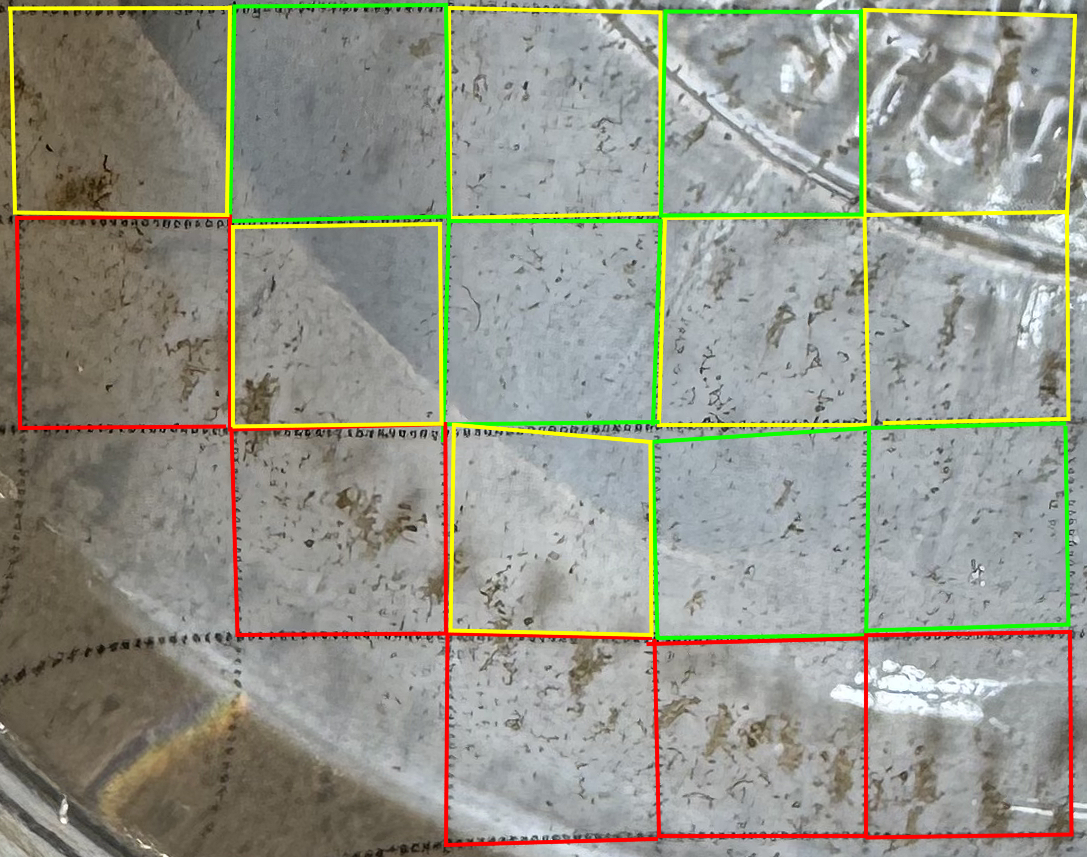
\includegraphics[width=1\linewidth]{Figures/BoxClasses}
		\caption[Box Classifications]{Annotated image showing the classifications of boxes based upon their particle counts.}
		\label{fig:boxclasses}
	\end{figure}
	\begin{figure}[h]
		\centering
		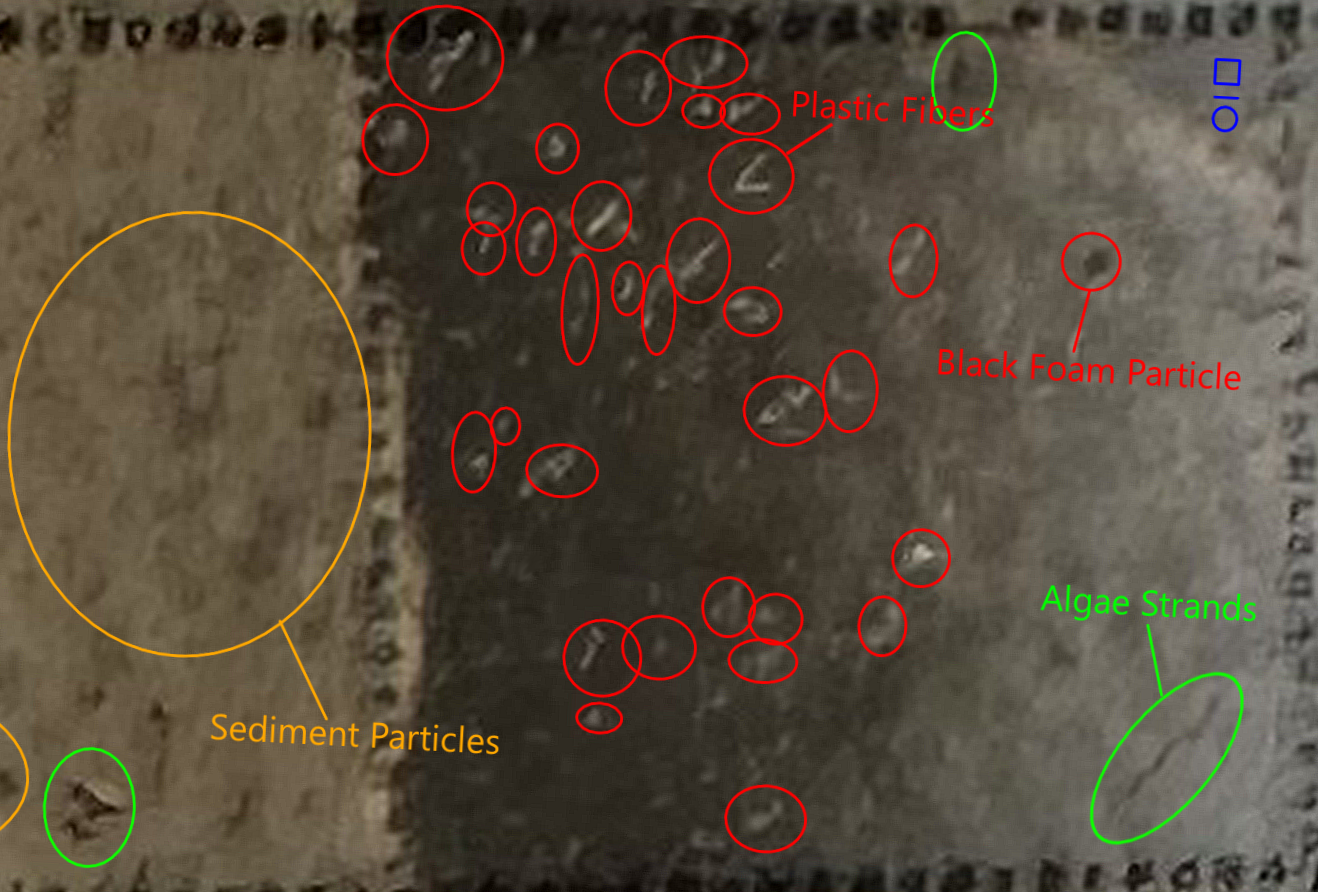
\includegraphics[width=1\linewidth]{Figures/MPsClassification}
		\caption[Annotated Collected Particles]{Annotated image showing how microplastics were differentiated from organic particles and sediments. Here, microplastics are circled in red, organics in green, and sediment in brown.}
		\label{fig:MPClassification}
	\end{figure}
	Note that not every particle thought to be a microplastic is marked in figure \ref{fig:MPClassification}, as it merely illustrates the application of selection criteria and not the actual counting of this region of particles. In the upper right hand corner, a square, line, and circle can be seen which denote the nominal smallest particle size which can be collected by the device. This is not necessarily the practical lower limit to size, as the filter used was double-layered for greater rigidity. The two layers were roughly aligned with each other, but some pores were still slightly smaller or larger than the nominal size. The filter on the other end of the output was also double-layered for consistency.
		\begin{figure}[h]
		\centering
		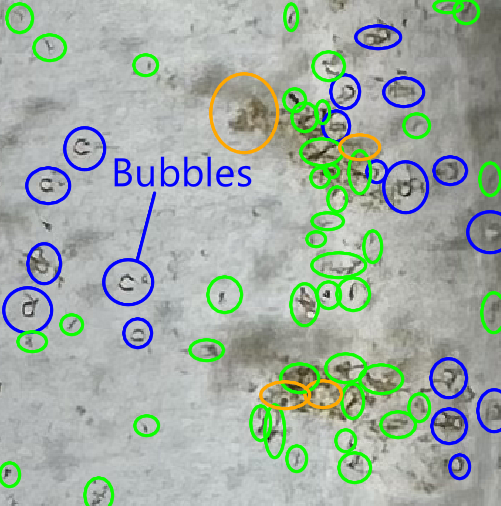
\includegraphics[width=1\linewidth]{Figures/OrganicsBox}
		\caption[Annotated Collected Organics]{Annotated image showing the output from the "release" end of the device. The classification criteria for this image is the same as in figure \ref{fig:MPClassification}, with the addition of bubbles. Many more bubble were present in the organic sample simply due to the mode of filtration being a simple filter as opposed to a rigid collection box.}
		\label{fig:OrganicsOutput}
	\end{figure}
}
	\fi
	\subsubsection{Collection Efficiency}
	\paragraph{Quantity and Numerical Proportions}
	To evaluate the efficiency of collection, samples were visually evaluated under a microscope to identify and count them. To ensure relatively random sampling, the sample which was intended to be collected (henceforth the MP sample) and the sample which would have otherwise been released into the river (henceforth the organic sample) were stirred with a metal rod, allowed to settle for approximately 5 minutes, then collected using a pipette and pipetted onto a slide. All tools which directly contacted the sample (such as the metal rod) were rinsed into the sample to minimize sample loss. This process was repeated 3 times to create 3 pseudo-random selections from each of the MP and organic sample, 6 in total. After slide preparation, random selections of the material on the slides were chosen by randomly turning the microscope's lateral movement dial and identifying each of the particles found within the aperture. Identification was carried out according to the guidelines in \ref{Huang_Hu_Wang_2022} At this stage, the only focus is \emph{quantity} of each particle type, thus certain sestons such as algae which tended to clump and form larger matrices typically including many algae cells, organic matter, and diatoms were counted as single particles. This reflects the fact that, for the purposes of filter feeding, mesobenthos and macrobenthos are unable to distinguish or separately process individual particles contained within these interlocked matrices. The process of counting, identifying, and moving was repeated for each slide until approximately 50 particles had been analyzed from each slide (n=166 for the MP sample, n=141 for the organic sample), with 307 particles analyzed in total. Once all particles were classified and counted, the data was compiled into figure \ref{fig:mpcounting}.
	\begin{figure}[h]
		\centering
		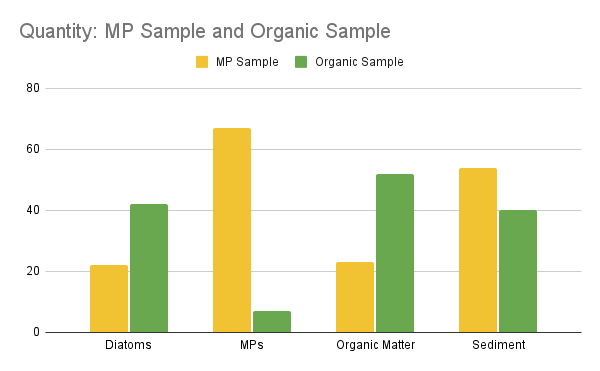
\includegraphics[width=1\linewidth]{Figures/MPOrganicCounting}
		\caption[Collected Particle Classification]{Bar chart with data of all particles collected in both the MP and organic samples.}
		\label{fig:mpcounting}
	\end{figure}
	
	As seen, the device collected just over 90\% of the microplastics which passed through it during the 4 hours of testing, strongly supporting goal \#2 of the Engineering Goals from section \ref{sec:goals}. Despite this success, goal \#3 of section \ref{sec:goals} was not met, with nearly 33\% of organic sestons being collected by the device. Given the importance of these organic particles to benthic ecosystems, this is unfortunate and may prevent the specific device used in this study from being used in more sensitive areas\textemdash though organic matter pass through efficiency could likely be improved by using higher quality, more expensive parts such as a 
	
	\begin{figure}[h]
		\centering
		
\includegraphics[width=1\linewidth]{Figures/RawSeparated}
		\caption[Raw Separated Plastics]{Raw, unprocessed particles extracted from the device's collection chamber directly after experimentation. Note that nearly all particles here are either beige colored sediment or white/clear plastic.}
		\label{fig:rawseparated}
	\end{figure}
	
	\begin{figure}[h]
		\centering
		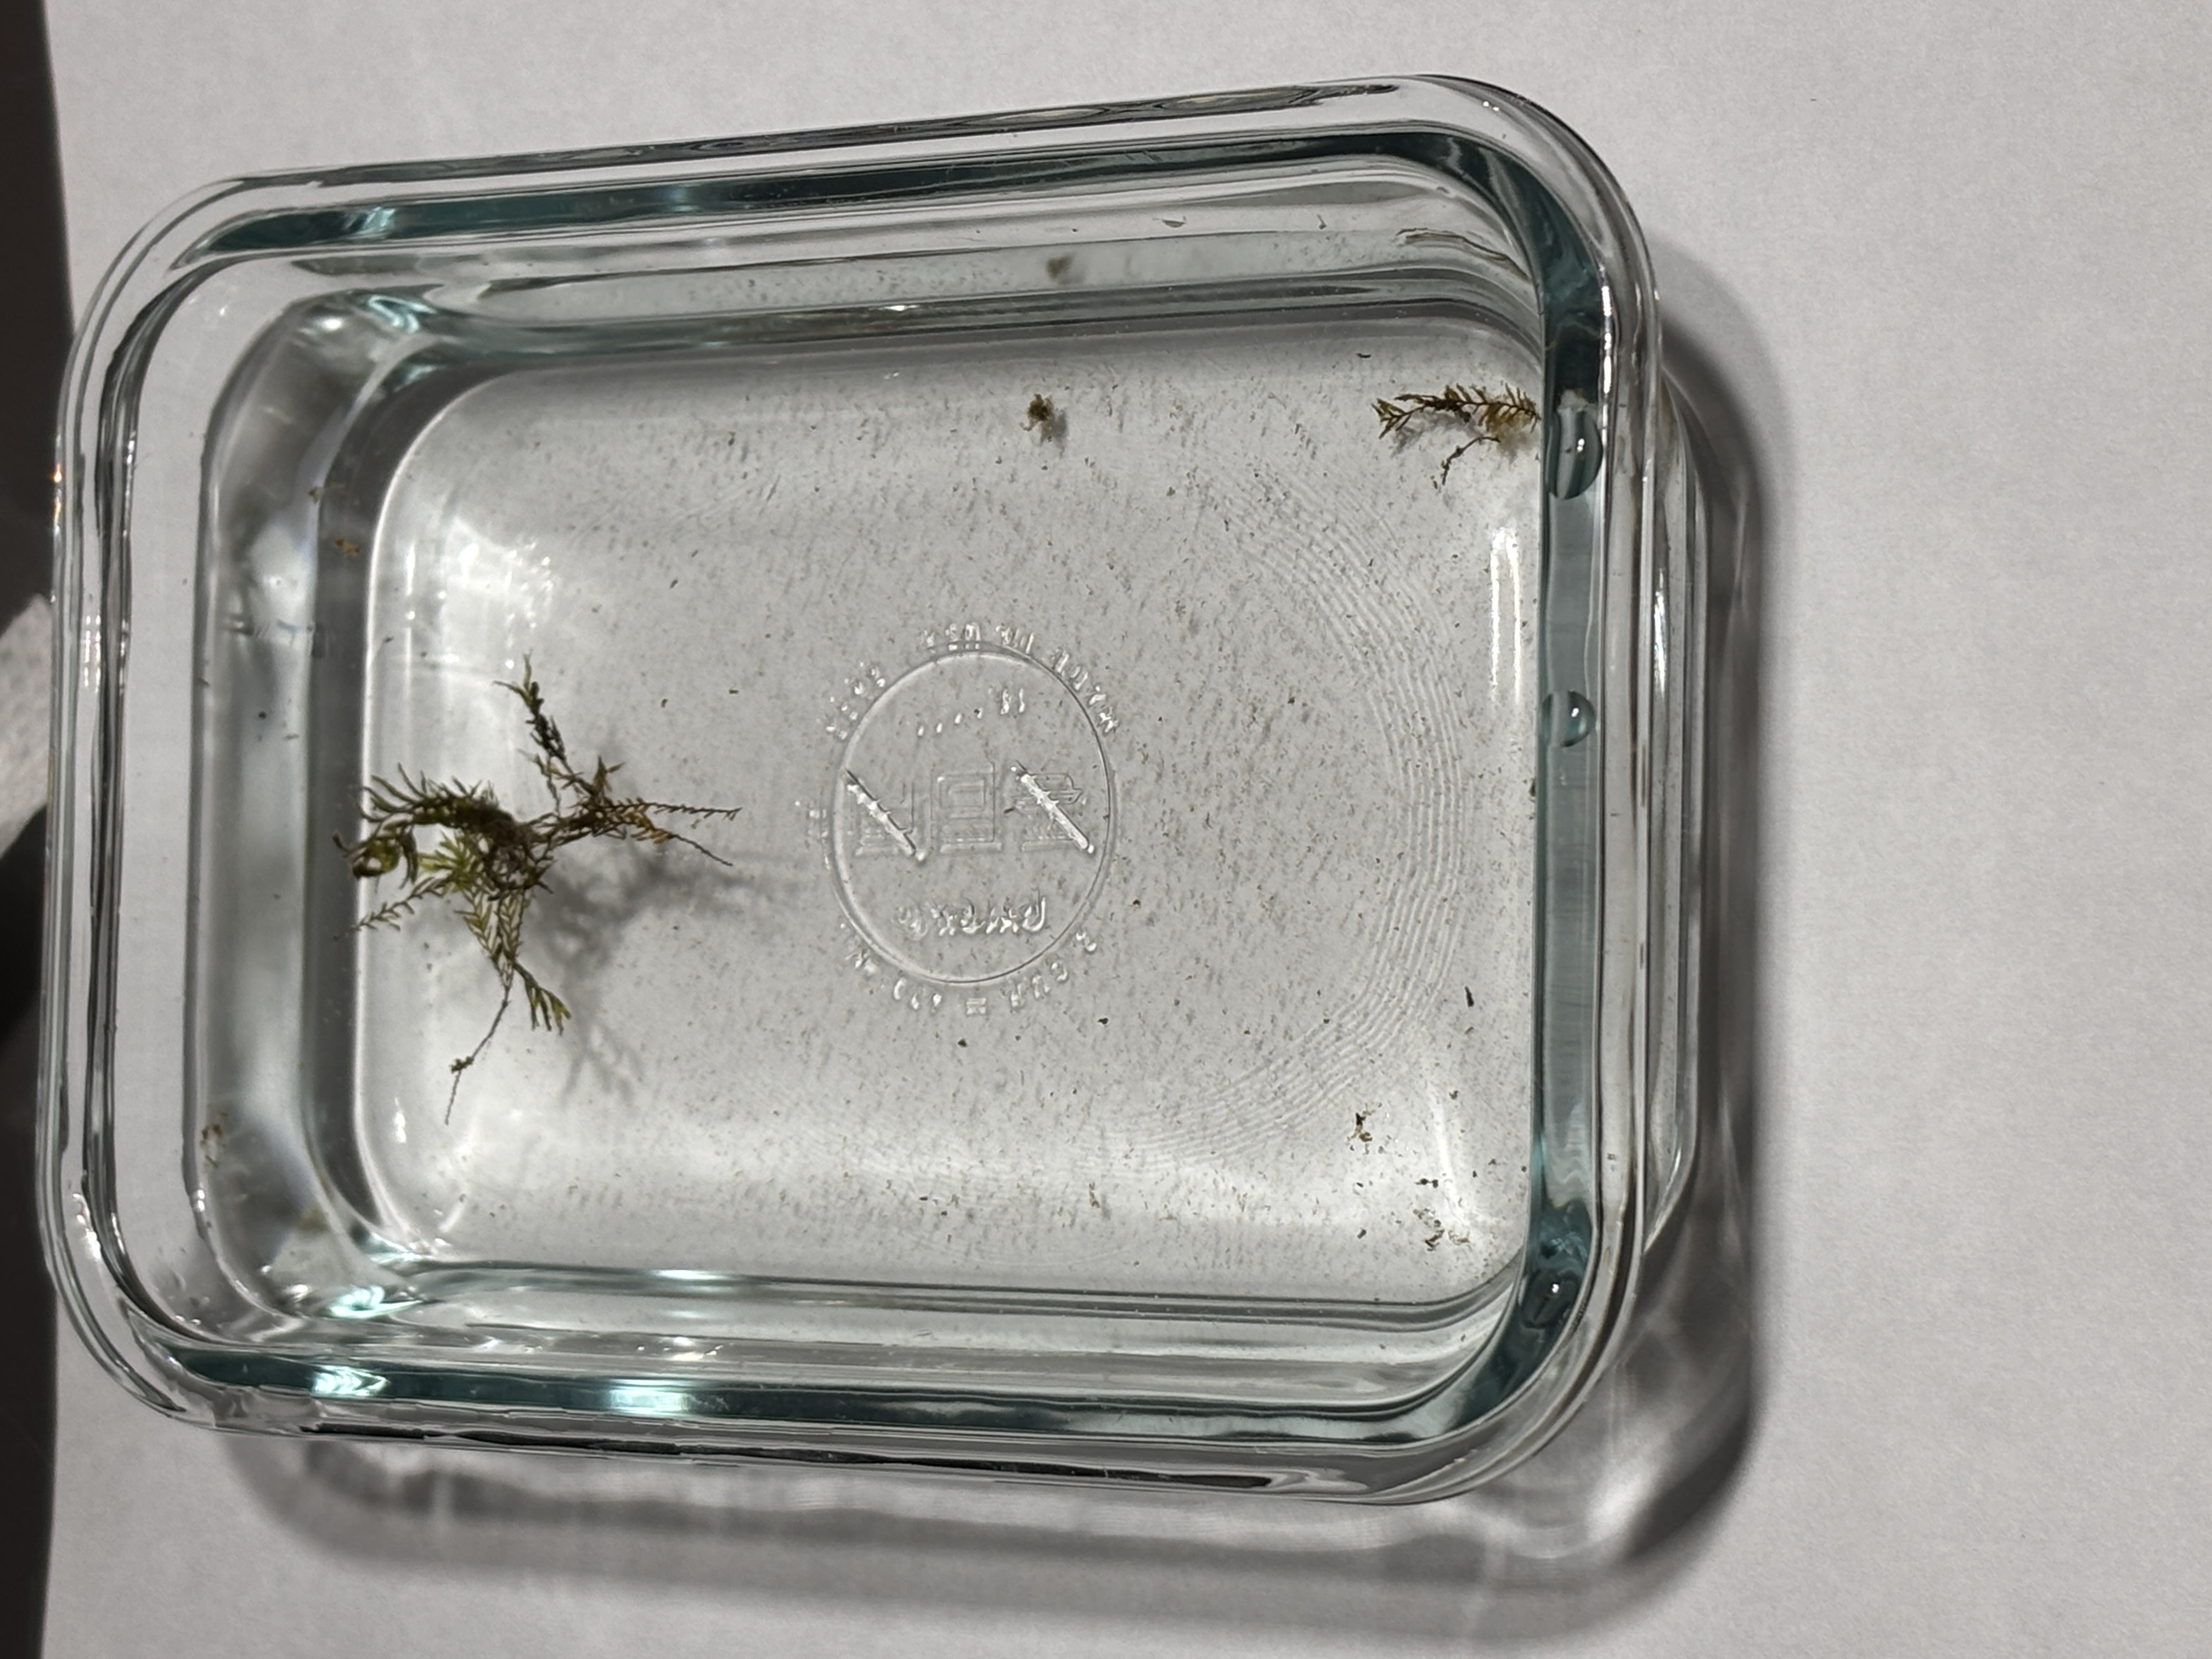
\includegraphics[angle=90,origin=c,width=1\linewidth]{Figures/RawReleased}
		\caption[Raw Released Particles]{Raw, unprocessed particles collected by a net on the "release" end of the device. Outside of an experimental scenario, these particles would be released back into the water column. Note the algae and green-ish particles which pervade this sample, and the comparatively very low number of easily visible plastic or sedimentary particles.}
		\label{fig:rawreleased}
	\end{figure}
	
	\subsubsection{Further Predictions}	
	If it is assumed that the Milwaukee River is relatively typical in its proportion of wash, bed, and suspended load, roughly 80\% of the 22.1 mg/L of total suspended load in the Milwaukee River, or 17.68 mg/L is likely the "wash load"\textemdash particles which stay permanently suspended and travel most of or the entire length of the river. Using the Milwaukee River's nominal length of 104 miles, the wash load should spend at most 3-4 days suspended assuming a river speed of $\approx$ 1-2 m/s. 
	\linebreak
	Using this information, it follows that removing microplastics in the wash load at various points in the river will remove significant portions of downstream microplastic pollution as shown in figure \ref{fig:washload}.
\begin{figure}[h]
	\centering
	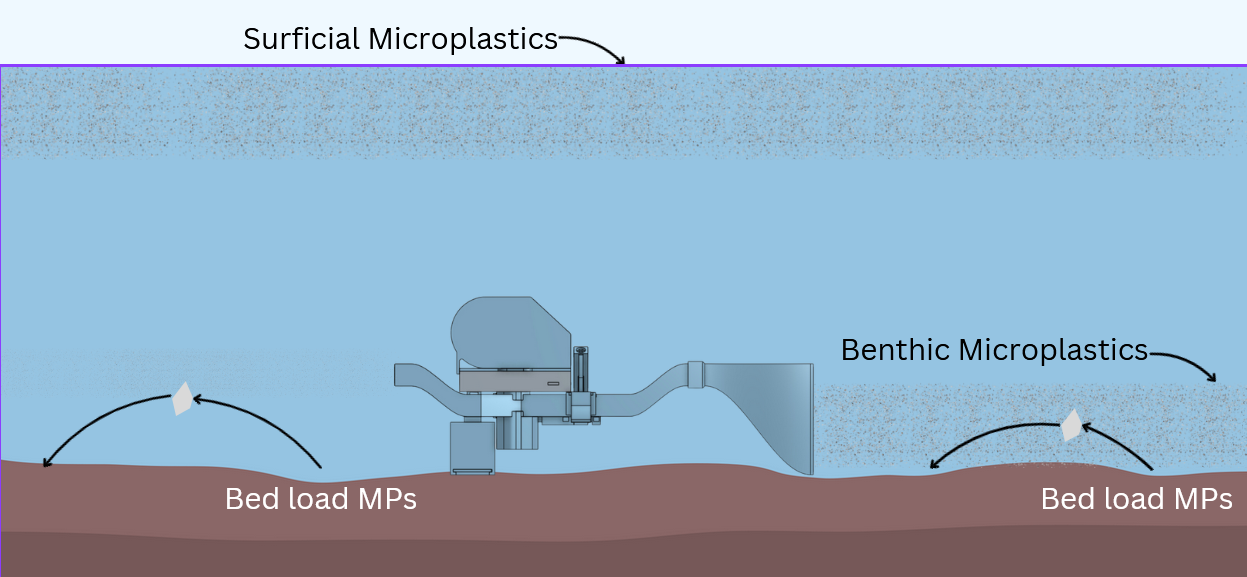
\includegraphics[width=1\linewidth]{Figures/WashLoadCollection}
	\caption[Wash Load MP Collection]{Illustration of how a single collection checkpoint can significantly lower downstream benthic microplastic concentrations.}
	\label{fig:washload}
\end{figure}
By using several of these "microplastic checkpoints" at various points throughout the river, MP concentrations at any given point in the river can be decreased very significantly with relatively little investment. Using the Milwaukee river as a model, placing 10 of these checkpoints at various points in the river could decrease microplastic concentrations at any given time by $\approx$52.8\% (88\% efficiency * 80\% wash load * 75\% margin)
	\subsection{Risks}
	Outside of the typical risks associated with existing and working within a workshop environment, this project poses very few dangers. The majority of parts for the final device are 3D printed or off-the-shelf components, not pieces which need to be separately manufactured via CNC, drilling, etc. Besides these standard risks, physically placing the device into the water during the empirical testing will likely be the most dangerous part of the project, however, this will be performed with others present and in water which only reaches $\approx$2-3 feet deep at maximum as seen in figure \ref{fig:riverCrosssec}. With proper attire (waders, gloves, jackets, etc.) this should not pose any significant risk.
	
	%------------------------------------------------
	
	\phantomsection
	\section*{Acknowledgments} % The \section*{} command stops section numbering
	
	\addcontentsline{toc}{section}{Acknowledgments} % Adds this section to the table of contents
	
	
	%----------------------------------------------------------------------------------------
	%	REFERENCE LIST
	%----------------------------------------------------------------------------------------
	
	\phantomsection
	%\bibliographystyle{apa}
	\bibliographystyle{unsrt}
	\nocite{*}
	\bibliography{sample.bib}
	
	%----------------------------------------------------------------------------------------
	
\end{document}
